% MUST use a4paper option
% MAY use twoside, smaller font, and other class
\documentclass[a4paper,12pt]{article}
% Use UTF-8 encoding in input files
\usepackage[utf8]{inputenc}
% NOTE: If you are writing in English, un-comment the following line:
% \usepackage[swedish,english]{babel}
% Use the template for thesis reports
\usepackage{UppsalaExjobb}
\usepackage{float}
\usepackage{cleveref}
% Useful font packages for maths and symbols
\usepackage{amssymb,amsmath,amsthm,amsfonts}

% for nice code listings
\usepackage{listings}

% Designval: per default används styckesindrag, men ibland blir det snyggare/mer lättläst med tomrad mellan stycken. Det åstadkoms av de följande raderna.
% Tycker ni om styckesindrag mera, kommentera bort nästa två rader.
\parskip=0.8em
\parindent=0mm

% Designval: vill ni ha en box runt figurer istället för strecken som är default, av-kommentera raden nedan. Obs att både \floatstyle och \restylefloat behövs.
%\floatstyle{boxed} \restylefloat{figure}

\begin{document}
% För att ställa in parametrar till IEEEtranS/IEEEtranSA behöver detta ligga här (före första \cite).
% Se se IEEEtran/bibtex/IEEEtran_bst_HOWTO.pdf, avsnitt VII, eller sista biten av IEEEtran/bibtex/IEEEexample.bib.
\bstctlcite{rapport:BSTcontrol}

% Set title, and subtitle if you have one
\title{Positioneringssystem för aktivitetsbaserade arbetsplatser} % och uppsatsmetodik
% Use this if you have a subtitle
%\subtitle{Really Exciting Stuff}
% Set author names, separated by "\\ " (don't forget the space)
% List authors alphabetically by last name (unless someone did significantly more/less)
\author{Alexander Backlund \\ Sebastian Gustafsson \\ Albin Hjelm }
% Set the date and year - use the right language!
\date{\begin{otherlanguage}{swedish}  %\foreignlanguage doesn't seem to affect \today?
\today
\end{otherlanguage}}

% Only need to set the year if it differs from the current year
%\year=2018

% Ange handledare, ämnesgranskare, examinator om dessa finns
% Extern handledare: t.ex på företag ni arbetat med?
%\exthandledare{NN}
% Intern handledare
\handledare{Lisa Lagom och Björn Victor}
% Ämnesgranskare används inte på Självständigt arbete i IT
%\reviewer{NN}
% På Självständigt arbete i IT är detta BV
\examinator{Björn Victor}

% Programnamn på svenska och engelska
\progname{Civilingenj{\"o}rsprogrammet i informationsteknologi}{Master Programme in Computer and Information Engineering}

% Utgivare
\enhetsnamn{Institutionen för \\ informationsteknologi}
\besoksadress{ITC, Polacksbacken\\ Lägerhyddsvägen 2}
\postadress{Box 337 \\ 751 05 Uppsala}
\hemsida{http:/www.it.uu.se}

% Set the name of the series, and the number in the series
\seriesname{Självständigt arbete i informationsteknologi}
% \seriesname{Uppsatsmetodik}

% OBS: Gäller bara exjobb i årskurs 5
% Get a series number, e.g. from Studentservice Ångström
%\seriesnumber{UPTEC IT16~0xx}
% Use the appropriate ISSN for the series
%\issn{ISSN 1401-5749}
% Usually this is where it is printed
%\printer{Ångströmlaboratoriet, Uppsala universitet}

% This creates the title page
\maketitle

% Change to frontmatter style (e.g. roman page numbers)
\frontmatter

\begin{abstract}
  % Abstract in English, about 10-20 lines. Do not use references; do not use formulas if they can be avoided.
  % \begin{enumerate}
  % \item What is the problem/issue/subject?
  % \item How was the problem solved/attacked?
  % \item What are the results, how well was the problem solved?
  % \item How good are the results, how useful are they?
  % \end{enumerate}
  % The abstract should be understandable without reading the whole report (and the rest of the report should be understandable without reading the abstract). You can reuse text/phrases from the Introduction.
  Many companies and organisations nowadays chose to transfer from an office structure consisting of employee dedicated offices, into having a more open and office free structure. With that transition some difficulties occur in locating coworkers when you want to meet them. This is because they now have the opportunity to choose workplace more freely. %work related concerns with%.
   Beacause of this, employees looses productivity and spends unnecessary time and energy on locating coworkers. This project's intent is to make this transition easy, non time consuming and available only by using existing information and technology at the workplace. This is to be provided via a location platform at which users can locate their co-workers. %TODO skriv hur väl vi löste problemet.
\end{abstract}

\begin{sammanfattning}
  % Sammanfattning på svenska. Se till att det står samma saker i det svenska och det engelska abstractet.
  % \begin{enumerate}
  % \item Vad är problemet, ämnet?
  % \item Hur angreps/löstes problemet?
  % \item Vad är resultaten, hur väl löstes problemet?
  % \item Hur bra blev resultaten, hur användbara är de?
  % \end{enumerate}
  %
  % Ca 10-20 rader. Använd inte referenser; ej heller formler om det går att undvika.
  %
  % Abstract ska vara förståeligt utan att läsa resten av rapporten, och resten av rapporten ska kunna läsas utan att läsa abstract. Man kan återanvända text från introduktionen.
  Många företag och organisationer väljer nuförtiden att övergå från en kontorsstruktur bestående av dedikerade kontorsplatser för var och en av medarbetarna, till en öppnare och mer kontorsfri struktur. %TODO kanske skriva om meningen då den är ganska lång, dock tycker jag om den...
  Med den övergången tillkommer vissa problem med att hitta enskilda medarbetare som du vill träffa eftersom de nu har möjlighet att välja arbetsplats friare. På grund av detta tappar de anställda i produktivitet eftersom de behöver spendera onödig tid på att lokalisera sina kollegor. En kontorsstruktur där medarbetarna väljer arbetsplats utifrån arbetsuppgift kallas för en aktivitetsbaserad arbetsplats. Det här projektets intention är att göra övergången till en aktivitetsbaserad arbetsplats enkel, icke tidskrävande och möjlig genom att endast använda befintlig teknik och information på arbetsplatsen. Medarbetarnas position presenteras via en lokaliseringsplattform där varje användare enkelt kan lokalisera sina medarbetare.
\end{sammanfattning}

% Innehållsförteckningen här.
\tableofcontents

% Här kan man också ha \listoffigures, \listoftables

\cleardoublepage


% Change to main matter style (arabic page numbers, reset page numbers)
\mainmatter

% Here comes the text of the report.
\iffalse
\section*{Hur ni använder detta malldokument}
Titta i källdokumentet för diverse inställningar för författare, titel, etc.

\emph{OBSERVERA} att de ``fasta fält'' som blir på svenska (trots att ni ställt in engelska med \texttt{babel}), som Examinator, Handledare, datum på framsidan osv, \emph{ska} vara på svenska oavsett språk i rapporten. Abstract ska alltid vara på engelska, medan Sammanfattning alltid ska vara på svenska.

I flera appendix finns mer info som inte gäller rapportstrukturen.

I era inlämningar, ta bort (eller kommentera bort) malltexten (beskrivningen av vad som ska stå), men behåll gärna tomma huvudrubriker. Ta också bort mall-appendix.

\subsection*{Generellt}
Varje numrerat avsnitt ska finnas med i er slutrapport, om inget annat anges.
Välj rubrik på svenska eller engelska beroende på ert valda rapportspråk.

Glöm inte att läsa kurslitteraturen~\cite{dawson:projects-in-computing,dawson:projects-in-computing-old}.

% \subsection*{Uppdateringar av detta dokument}
% \begin{description}
% \item[2016-05-16]\mbox{}\\

% \end{description}

 %%%%%%%%%%%%%%%% OBS! Ta bort allt mellan \mainmatter och här (inkl \newpage) i slutversionen (men inte \mainmatter)
\fi
 \section{Introduktion}
 \iffalse Beskriv åtminstone samma saker som i abstract, men mer utförligt. Spara tekniska detaljer till senare.

 Tänk på att börja introduktionen med en mening eller ännu hellre ett helt stycke som ``fångar'' läsaren och motiverar läsaren att fortsätta läsa.  \emph{Vi har valt att göra ett projekt om X} är relevant för er, men kommer inte att vilja få någon att läsa vidare.  Försök åtminstone få med någon slags bakgrund/kontext och (helst) motivation att fortsätta läsa.  Typ \emph{X är ett programspråk som tagit världen med storm.  Vi vill utforska om man kan kombinera X med Y för att göra\ldots}

 Se till att ni \emph{kommer till kritan snabbt} – man vill inte läsa igenom två stycken text innan man får veta vad ni tänker göra i ert projekt.  Börja t.ex. \emph{inte} med att presentera alla idéer ni inte valt – läsaren vill veta vad ni ska göra, inte vad ni inte ska göra.

 Översiktlig beskrivning av systemet och dess features ska vara under systemdesign / systemstruktur, inte i introduktionen.

 Introduktionen bör vara begriplig för t.ex.~en student i årskursen under, och gärna för en ännu bredare läsarkrets.
 \fi

 Fler och fler företag och organisationer väljer idag att övergå från kontorsbaserade till aktivitetsbaserade arbetsplatser. Iden med en aktivitetsbaserad arbetsplats är att arbetsytorna öppnas upp och delas in i områden snarare än mindre kontor. Ett problem med denna typ av miljö är att det är svårt att veta var sina medarbetare befinner sig. En lösningen till detta problem är systemet som presenteras i denna rapport.

 Systemet fungerar på sätt att när en medarbetare väljer en arbetsplats och startar sin dator kommer datorn att skanna av nätverksinformationen i närheten och bestämma medarbetarens position. Denna position kommer att visas på en hemsida så att andra medarbetare snabbt kan se var sina kollegor befinner sig. Som användare finns även möjligheten att välja att inte visa sin position.

 Systemet i sin helhet består dels av en mobilapplikation som används för att i förhand registrera information om den befintliga nätverksmiljön på arbetsplatsen. Denna information behövs i ett senare skede då en enskild användare ska positionsbestämmas. Systemet består även av ett program som varje användare av systemet kommer att köra på sin egna dator. Detta program använder informationen genererad av mobilapplikationen för att positionsbestämma användaren. Efter  att programmet positionsbestämt en användare skickar programmet användarens position till en datorbas. Slutligen består systemet även av en hemsida som alla användare av systemet har tillgång till. På hemsidan har användare möjlighet att se var andra användare befinner sig. %TODO BEhövs detta, känns överflödigt men det förtydligar vad alla delar gör vilket var en feedback punkt. Man kan även ta upp lite resultat här antar jag.

 Systemet kan positionera en användare utifrån vilket våningsplan de befinner sig på med en träffsäkerhet på 100\% i de lokaler som testerna utfördes i. Systemet kan också positionera en användare inom ett områden på samma våningsplan med en träffsäkerhet på fem meters marginal. Om en användare befinner sig mindre än fem meter in i ett specificerat område positionerar systemet i vissa fall användaren till det angränsande området.


 \section{Bakgrund}
 I bakgrunden förklaras först vad som menas med en aktivitetsbaserad verksamhet (ABV). Därefter beskrivs detta projekts externa intressent, Uppsala kommun. Uppsala kommun har under de senaste åren påbörjat en övergång till ABV. Uppsala Kommun använder i sin dagliga verksamhet Skype for business (SFB) som kommunikationsverktyg och har uttryckt ett önskemål om att kunna integrera ett positioneringssystem i SFB. SFB beskrivs utförligare i sektion \ref{SFB} nedan. Därefter tas några problem upp som gäller specifikt för inomhuspositionering. Avslutningsvis redogörs för vissa icketekniska aspekter som vi har tagit hänsyn till under utvecklingen av detta system.


 \subsection{Aktivitetsbaserad verksamhet}
 Madeleine Stjärne, författaren till skriften ``Aktivitetsbaserade
 arbetsplatser i offentlig sektor''\cite{ABV}, beskriver aktivitetsbaserade arbetsplatser på så sätt att de erbjuder medarbetare en varierad arbetsmiljö. Hon hävdar att syftet med ABV är att medarbetare inte ska behöva vara bundna till ett specifikt skrivbord utan istället kunna välja den mest ändamålsenliga arbetsplatsen utifrån den aktuella arbetsuppgiften. % variationen för den individa arbetaren.

 Då en organisation väljer att övergå till en aktivitetsbaserad arbetsplats
 delas arbetsplatsen in i olika miljöer som stödjer de olika arbetsuppgifterna som ska utföras, såväl individuella arbeten som grupparbeten. En sådan uppdelning görs baserat på resultatet av en verksamhetsanalys. I en verksamhetsanalys analyseras hur arbetsplatsen har använts tidigare. De viktigaste parametrarna att undersöka vid en verksamhetsanalys är vilka arbetsuppgifter som utförs, var de utförs och hur ofta de utförs \cite{ABV}.
 Det är vanligt att arbetsplatsen delas upp i olika zoner. Exempel på zoner kan vara tysta zoner och möteszoner. Medarbetarna söker sig då till den zon de tycker passar bäst för dagens arbete.

 Enligt Lisbeth Slunga Järvholm, forskare vid Umeå universitet, passar inte ett aktivitetsbaserat kontor alla. Inte alla sorters arbetsuppgifter fungerar optimalt då arbetarna lätt kan bli störd. Vissa arbetsuppgifter kräver en högre koncentrationsnivå, vilket kan vara svårt i ett öppet kontorslandskap \cite{passarInteAlla}.
 %TODO Fördelar med ett aktivitetsbaserat kontor

 \subsection{Uppsala Kommun}
 Uppsala Kommun agerar i det här projektet extern intressent. De är i ett skede där de övergår till aktivitetsbaserade arbetsplatser på många av deras kontor runt om i Uppsala. Det innebär att
 ett par tusen personer kommer att kunna välja friare var de vill utföra sina arbetsuppgifter. Uppsala Kommun har uttryckt ett behov av att deras medarbetare snabbt ska kunna se var deras kollegor befinner sig. Det är vår förhoppning att de ska kunna utnyttja det här systemet för att kunna uppfylla deras behov.
 \iffalse
 \subsection{Inomhuspositionering}
 Inomhuspositionering är jämfört med utomhuspositionering ett problem med fler komplikationer. GPS-tekniken(Global Position System) som ger en mycket liten felmarginal vid utomhuspositionering är sällan användbar för inomhuspositionering. Anledningen är att GPS-tekniken kräver en oblockerad signal till de satelliter som GPS använder sig av för positionsbestämning \cite{GPS_US_ACCURACY}.

 I fallet med inomhuspositionering i kombination med en aktivitetsbaserad arbetsplats ser kraven på precision något annorlunda ut jämfört med precisionskraven för utomhuspositionering. Även om GPS-tekniken kan användas för att bestämma en enhets höjd över marken är den inte tillräckligt tillförlitlig för att bestämma vilket våningsplan enheten befinner sig på.

 En av skillnaderna är att det vid positionsbestämning inomhus tillkommer en faktor som komplicerar positionsbestämningen. Problemet är att vid inomhuspositionering måste ta hänsyn till ett visst antal våningsplan i en byggnad. Även om GPS-tekniken skulle kunna leverera lika god precision inomhus som utomhus (i förhållande till ett globalt koordinatsystem) skulle detta vara otillräckligt i och med att informationen inte anger huruvida den fastställda enhetens position befinner sig på våning 1 eller 15.
 %TODO Säger du typ inte samma sak här som på förra stycket?\subsection{Problem med GPS-tekniken}
 Vid utomhuspositionering har GPS-tekniken utgjort en generell möjlighet till att bestämma en position med i de flesta fall godtagbar precision, ca 4 meters felmarginal\cite{GPS_US_ACCURACY}.
 Global Positioning System (GPS) är en teknik som ägs av den Amerikanska staten och underhålls av USA:s flygvapen. GPS är ett system bestående av 24 satelliter som kretsar kring Jorden. Satelliterna sänder ut radiosignaler med information
 om deras position och en exakt tidpunkt då de sänder signalen. Mottagare i form av smartphones och liknande apparater fångar upp signaler från de satelliterna som befinner sig inom räckhåll och använder sig av satelliternas tid och plats-information för att med hjälp av geometri avgöra var på planeten de befinner sig \cite{GPS_US_HOW}.

 Problemen med GPS-tekniken är att precisionen försämras då mottagarna befinner sig i närheten av byggnader. Anledningen är enligt National Coordination Office for Space-Based Positioning att signalerna från satelliterna reflekteras när de kommer i kontakt med byggnader. De anser inte GPS-positionering som tillförlitlig då mottagaren befinner sig inomhus eller under jord \cite{GPS_US_ACCURACY}. Detta gör att andra tekniker måste användas för inomhuspositionering.
 \fi
 \subsection{Skype for Business}\label{SFB}
 SFB är ett kommunikationsmedel som används av många företag och organisationer. SFB erbjuder funktionalitet såsom realtidssamtal, videomöten och chattfunktioner. SFB kommer med en möjlighet att konfigurera en egen platsdatabas på SFBs server \cite{Microsoft-Office}. Det är en funktion som har undersökts om den är lämpligt att använda i detta projekt. När SFBs platsdatabas är populerad med nätverksinformation för varje område på organisationens arbetsplatser kan en medarbetares position bestämmas med hjälp av vilket nätverk medarbetaren är ansluten till. Denna information visas under användarens namn i SFBs användargränssnitt och är då synlig för andra Skypeanvändare i samma SFB-organisation. Detta gör att användare i SFB enkelt kan lokalisera varandra.

 Skype erbjuder två olika versioner av tjänsten SFB. Den ena varianten, SFB \textit{Online} är en molnbaserad tjänst som inte kräver några fysiska servrar hos användaren\cite{SFBonline}.
 Den andra varianten, SFB \textit{Server} kräver fysiska servrar hos användaren\cite{SFBserver}. Funktionaliteten för de två olika versionerna skiljer sig delvis åt och intressenten i det här projektet (Uppsala Kommun) hade som önskemål att det utfördes en undersökning huruvida funktionaliteten med en platsdatabas i SFB var möjligt i deras fall. Uppsala kommun använder SFB Online.



 \subsection{Problem med GPS-tekniken}
 Vid utomhuspositionering har GPS-tekniken utgjort en generell möjlighet till att bestämma en position med i de flesta fall godtagbar precision, ca 4 meters felmarginal\cite{GPS_US_ACCURACY}.
 Global Positioning System (GPS) är en teknik som ägs av den Amerikanska staten och underhålls av USA:s flygvapen. GPS är ett system bestående av 24 satelliter som kretsar kring Jorden. Satelliterna sänder ut radiosignaler med information
 om deras position och en exakt tidpunkt då de sänder signalen. Mottagare i form av smartphones och liknande enheter fångar upp signaler från de satelliter som befinner sig inom räckhåll och använder sig av satelliternas tid och plats-information för att med hjälp av geometri avgöra var på planeten de befinner sig \cite{GPS_US_HOW}.

 Problemen med GPS-tekniken är att precisionen försämras då mottagarna befinner sig i närheten av byggnader. Anledningen är enligt National Coordination Office for Space-Based Positioning att signalerna från satelliterna reflekteras när de kommer i kontakt med byggnader. De anser inte GPS-positionering som tillförlitlig då mottagaren befinner sig inomhus eller under jord \cite{GPS_US_ACCURACY}. Detta gör att andra tekniker måste användas för inomhuspositionering.


 %\subsection{Dataskyddsförordningen}
 %https://www.datainspektionen.se/dataskyddsreformen/dataskyddsforordningen/introduktion-till-dataskyddsforordningen/ TODO: skriv om detta!
 \subsection{Icketekniska aspekter vid inomhuspositionering på \\arbetsplatser}\label{icketekniska_aspekter}

 \subsubsection{Säkerhetsmässiga aspekter}
 Då många företag och organisationer har säkerhetsmässiga överväganden att ta hänsyn till är det viktigt att systemet inte bidrar till att säkerheten för medarbetarna i en organisation försämras vid användning av systemet.
 Då systemet har som uppgift att göra det lättare att lokalisera personal på arbetsplatser kan säkerhetsrisker uppstå. Om det är möjligt för utomstående personer att ta del av information om var personal befinner sig kan det leda till säkerhetsproblem. I Uppsala kommuns fall finns ett konkret exempel på den typen av säkerhetsproblem. Det arbetar många politiker inom Uppsala kommun och politiker är en yrkesgrupp som ofta får motta våld eller hot om våld. Ifall systemet bidrar till att det går att tillskansa sig deras exakta position utsätter systemet eventuellt dem för risker som inte skulle uppstå utan systemet.

 %TODO flytta till diskussion
 Detta innebär att det i systemet är viktigt att det är möjligt att välja att inte visa sin position för andra. Det är också viktigt att personer utanför organisationen inte kan ta del av information om var personal befinner sig.

 \subsubsection{Etiska aspekter}
 Ur ett etiskt perspektiv finns också vissa frågeställningar som blir viktiga att ha i åtanke under systemets utveckling. Ska systemet till exempel göra det möjligt att öka kontrollen över medarbetarna genom att deras position alltid är känd? Är det lämpligt att föra statistik över var medarbetare befinner sig vid olika tidpunkter?

 %TODO flytta till diskussion
 Målet med det här systemet är inte att det ska användas som ett maktmedel utan för att underlätta för medarbetarna.

 \subsubsection{General Data Protection Regulation, GDPR}\label{GDPR}
 GDPR är en ny Europeisk Lagstiftning som gäller alla medlemsländer i EU och träder i kraft den 25 maj 2018.
 Lagstiftningen reglerar hantering av personuppgifter och har som syfte att stärka individens rättigheter då företag och organisationer hanterar personuppgifter \cite{GDPRibm} \cite{GDPRdatainspektionen}.
 Individer har nu rätt att ta ett ärende som gäller personuppgiftshantering till en rättsprocess mot företag som de anser ha brutit mot de krav som GDPR innebär.
 Myndigheten Datainspektionen i Sverige har nu möjlighet att utdela böter till organisationer och företag som de anser bryter mot de nya lagarna. Det högsta bötesbeloppet som kan utdömas är 4\% %TODO 4% av VAD???
 eller 20 miljoner Euro \cite{GDPRibm}.

 GDPR eller Dataskyddsförordningen på svenska har vissa regler som i Sverige sedan tidigare reglerats i personuppgiftslagen (PUL). De likheter som finns är bland annat kravet på samtycke och rätten för en individ att få ta del av hur personuppgifter behandlas. PUL utgår den 25 maj 2018 i sin helhet och ersätts av GDPR \cite{GDPRdatainspektionen}.

 Några av de viktigaste nyheterna som detta innebär för den enskilda individen är enligt Datainspektionen\cite{GDPRdatainspektionen}:
 \begin{itemize}
   \item Dataportabilitet
   \item Konsekvensbedömning innan hantering
   \item Anmälningsskyldighet för organisationen
   \item Dataskyddsombud hos organisationen
   \item Sanktionsavgifter vid överträdelse
   \item Missbruksregeln upphör.
 \end{itemize}

 Nedan följer Datainspektionens \cite{GDPRdatainspektionen} förtydligande gällande ovan nämnda begrepp.

 \textbf{Dataportabilitet} innebär att individer ska ha rätten att få ut de personuppgifter de lämnat för att kunna flytta de till en annan tjänst.

 \textbf{Konsekvensbedömning} innebär att innan någon planerar att hantera personuppgifter ska det undersökas vilka risker hanteringen skulle kunna innebära för individen och hur dessa risker ska kunna förebyggas.

 \textbf{Anmälningsskyldighet} innebär att vid dataintrång eller dataförlust måste de drabbade informeras och en anmälning måste göras till Datainspektionen inom 72 timmar.

 \textbf{Dataskyddsombud.} Innebörden av kravet på ett dataskyddsombud är att varje företag eller organisation som hanterar känsliga personuppgifter måste ha ett dataskyddsombud som hanterar frågor gällande dataskydd.

 \textbf{Sanktionsavgift} innebär att Datainspektionen vid överträdelse av dessa regler har rätt att utdela böter i förhållande till hur allvarlig överträdelsen anses vara.

 \textbf{Missbruksregeln} är en regel som funnits i PUL och har inneburit att vissa personuppgifter får behandlas så länge de inte anses kunna vara kränkande för någon. Denna regel försvinner i och med att GDPR börjar gälla.

 Enligt en av IT-strategerna hos Uppsala Kommun innebär den nya lagen att många företag och organisationer, inklusive Uppsala Kommun, kommer behöva genomgå ett omfattande arbete för att säkerställa att de nya kraven för hantering av personuppgifter uppfylls.
 Därmed har det också varit vår avsikt att systemet ska uppfylla alla de krav på personuppgiftshantering som den nya lagen ställer.
 %TODO flytta till diskussion
 Den kritiska delen i projektet är att sambandet mellan en person och en plats kommer lagras i en databas och sedan presenteras för deras kollegor.
 Därför bör alla anställda dels kunna välja att inte finnas med i systemet över huvud taget och dels kunna välja att deras plats inte ska visas för andra. De personuppgifter som då hanteras är namn och avdelning på arbetsplatsen. Då systemet ställer dessa krav på samtycke uppfylls kraven mot GDPR i det avseendet.

 \subsubsection{Fackliga aspekter}
 Under ett möte med en företrädare för Uppsala Kommun uppkom även frågan om hur Fackförbunden kan tänkas ställa sig till att medarbetares position registreras.
 Denna frågeställning är svår att besvara. Den slutsats som drogs var att oavsett hur olika fackförbund kan komma att ta ställning till registrering av medarbetares position så innebär det att det är en frågeställning som bör reflekteras över när systemet designas.

 %TODO Flytta till  diskussion
 Eftersom möjligheten för personal att överhuvudtaget inte använda sig av systemet så borde eventuella fackliga problem kunna minska. Det är vår ståndpunkt att valfriheten för medarbetare och personal att använda systemet är ett val som måste erbjudas av företagsledningen eller organisationsledningen. Därmed blir också eventuella fackliga hinder en fråga för de personer i organisationen som eventuellt beslutar om användningen av systemet.



 %Här beskriver ni bakgrunden till ert projekt, d.v.s., det som leder fram till er %problemformulering.  Vilket är området, omgivningen, kontextet, bakgrunden för %projektet?  Beskriv området (t.ex. ljudbehandling, studieplaner, visualisering, %autism...).  Beskriv uppdragsgivare, om ni har (men inte för detaljerat).  Tänk %på att bakgrunden och problemet måste vara på en generell akademisk nivå och %inte bara relaterat till en uppdragsgivare.

 %Tänk på att bakgrunden kan se längre tillbaka -- hur löste man problemet förr? Ibland är det både viktigt och intressant (men ibland inte).

 %Efter att ha läst bakgrunden ska det vara uppenbart/lätt att förstå att syfte/mål är viktiga.

 \section{Syfte, mål, och motivation}\label{syfte_mal_mot}
 \iffalse
 Syftet med det här projektet är att utveckla ett enkelt och effektivt positioneringssystem för företag och organisationer som vill övergå till ABV. Systemet ska möjliggöra för medarbetare att enkelt kunna se var deras kollegor befinner sig.


 I första hand ämnar vi att undersöka huruvida det är möjligt att utveckla ett system som går att integrera med SFB. SFBs roll blir isåfall att vara den del av systemet som presenterar information om var användare befinner sig. Visar det sig att en integration med SFB inte är genomförbar är andrahandsalternativet att utveckla ett separat system för att presentera informationen.


 \subsection{Syfte}
 \fi
 Syftet med det här projektet är att utveckla ett enkelt och effektivt positioneringssystem för företag och organisationer som vill övergå till ABV. Systemet ska möjliggöra för medarbetare att enkelt kunna se var deras kollegor befinner sig. Projektet motiveras av att många företag och organisationer övergår till ABV. Uppsala Kommun har påbörjat en sådan övergång och har uttryckt ett behov av att medarbetare snabbt och enkelt ska kunna se var deras kollegor befinner sig. Uppsala kommun har arbetsplatser på ett flertal adresser runt om i Uppsala och upplever för tillfället det som ett problem att medarbetare har svårt att lokalisera varandra.
 Uppsala Kommuns medarbetare använder sig av SFB som kommunikationsmedel (se sektion ~\ref{SFB}) och har framfört ett önskemål att det direkt i SFB-applikationen ska gå att se var en medarbetare befinner sig.

 Målet är att erbjuda ett system som såväl Uppsala Kommun som andra företag och organisationer som vill övergå till ABV ska kunna använda sig av. Systemet ska vara enkelt att introducera, enkelt att använda och enkelt att underhålla.
 I första hand ämnar vi att undersöka huruvida det är möjligt att utveckla ett system som går att integrera med SFB. SFBs roll blir isåfall att vara den del av systemet som presenterar information om var användare befinner sig. Visar det sig att en integration med SFB inte är genomförbar är andrahandsalternativet att utveckla ett separat system för att presentera informationen.

 Målsättningen i ett prestandamässigt avseende är att användarna, då systemet är integrerat på arbetsplatsen, ska kunna se på vilken adress, vilken våning och i vilket område på den våningen som en kollega befinner sig. Uppsala Kommun har önskat en precision med max 10 meters felmarginal.

 \iffalse
 \subsection{Motivation}
 Projektet motiveras av att många företag och organisationer övergår till ABV. Uppsala Kommun har påbörjat en sådan övergång och har uttryckt ett behov av att medarbetare ska kunna se var deras kollegor befinner sig.

 Uppsala kommun har arbetsplatser på ett flertal adresser i Uppsala och beroende på arbetsuppgift ska arbetarna själva kunna bestämma var de vill utföra sina arbetsuppgifter.

 Uppsala Kommuns medarbetare använder sig av SFB som kommunikationsmedel och har framfört ett önskemål att det direkt i SFB-applikationen ska gå att se var en medarbetare befinner sig.


 \subsection{Mål}\label{mal}
 Målet är att erbjuda ett system som såväl Uppsala Kommun som andra företag och organisationer som vill övergå till ABV ska kunna använda sig av. Systemet ska vara enkelt att introducera, enkelt att använda och enkelt att underhålla.

 Målsättningen i ett prestandamässigt avseende är att då systemet är integrerat på arbetsplatsen ska användarna kunna se på vilken adress, vilken våning och i vilket område på den våningen som en kollega befinner sig. Uppsala Kommun har önskat en precision med max 10 meters felmarginal. Även om bättre precision än så inte anses vara nödvändig hoppas vi kunna uppnå en felmarginal på maximalt 5 meter. Målet är också att erbjuda en möjlighet för alla medarbetare att via en webbapplikation kunna se hur många medarbetare som befinner sig på en specifik arbetsyta. Webbapplikationens syfte är att göra det enkelt för medarbetarna att välja arbetsplats genom att kunna se var det finns lediga platser utan att fysiskt behöva gå igenom varje lokal och leta.
 %TODO ibland säger vi att webbapplikationen inte kommer användas av arbetarana och ibland säger vi att dom kommer använda det.
 \fi

 Vår förhoppning är att det här systemet ska kunna lösa några av de praktiska problem som uppstår för företag och organisationer som övergår till aktivitetsbaserade arbetsplatser. Förhoppningsvis kan detta också leda till att företag som överväger att övergå till ABV kommer känna mindre oro över att det dagliga arbetet behöver störas av problem med att hitta sina medarbetare.

 \iffalse
 Det finns sedan tidigare andra system som erbjuder inomhuspositionering. Vissa av dessa använder sig av extra hårdvara såsom Bluetooth Beacons. Vid användning av Bluetooth Beacons installeras först bluetoothenheter runt om på arbetsplatsen. Därefter sker positionsbestämningen med hjälp av analys av signaler från dessa Beacons(enheter).
 För att göra systemet attraktivt ska system inte kräva extra hårdvara och inte heller kräva nya applikationer för användarna. Systemet ska istället använda medel och teknik som redan finns på arbetsplatserna, framförallt trådlösa internetanslutningar.
 \fi
 %\label{sec:syfte}
 %Här beskriver ni i princip er problemformulering.  I detta avsnitt ska framgå syfte, mål, och motivation med projektet.
 %Dessa behöver dock \emph{inte} vara separata underrubriker.

 %\paragraph{Syfte.} Vart strävar projektet? vad är det övergripande målet, nyttan, effekterna av projektet?  (t.ex. bättre koll på kosthållning, enklare planering av studier\ldots)
 %\paragraph{Mål.} Vad ska konkret levereras/utföras av projektet, för att ta oss närmare syftet?
 %\paragraph{Motivation.}  Varför är projektet viktigt?  Vilka är det viktigt för, vilka externa intressenter finns?  Hur stort är problemet, vad är följden av att det inte är löst, hur bra vore det att lösa?  Vilken ``lucka'' i området täcker ni?
 %Varför är er lösning bättre/annorlunda än andras?

 %Se till att ni i detta avsnitt övertygar läsaren om att problemet finns, att det inte är löst, och att det är viktigt att lösa. Ju starkare argumentation och motivation (med källor) dess bättre.
 %\begin{itemize}
 %\item Visa att det finns ett problem.
 %\item Visa att problemet är viktigt att lösa, att det behöver lösas.
 %\item Visa att problemet inte redan är löst.
 %\end{itemize}

 \section{Avgränsningar}
 På grund av begränsad tid har vissa avgränsningar skett. Systemet använder endast fingerprintingtekniken för positionsbestämning (se sektion \ref{fingerprinting}). Det finns ytterligare tekniker som skulle kunnat användas i kombination med fingerprintingtekniken, till exempel trilateration (se sektion \ref{triangulering}).

 För att utföra positionsbestämning med hjälp av referenspunkter (se sektion \ref{referenspunkter}) så exakt som möjligt bör, enligt J. Jun m. fl., varje geografisk plats representeras med fler än en referenspunkt\cite{jun2018low}.
 Anledningen till detta är att olika typer av nätverkskort kan utläsa olika RSSI-värden (se sektion \ref{RSSI}) mot samma åtkomspunkt\cite{problem_with_RSSI}. Om varje planerad plats för en referenspunkt representeras med fler referenspunkter baserade på mätningar utföra av enheter med olika typer av nätverkskort kan det därmed fungera som en kompensation för att olika nätverkskort kan generera olika RSSI-värden\cite{jun2018low}.
 %TODO bra mening men väldigt lång.

 Ytterligare en avgränsning är att mobilapplikationen endast fungerar för Androidtelefoner.
 Avgränsningen med att endast utveckla scanningsapplikationen för Android gjordes dels på grund av tidsbrist med också eftersom applikationen endast kommer att användas ett fåtal gånger, dvs då systemet installeras på arbetsplatsen. Vi ansåg att det var lämpligare att utveckla applikationen för Android eftersom det är enklare och smidigare att publicera en Andoidapplikation än till exempel en Iphoneapplikation. Den enda åtgärden som krävs för att publisera en Androidapplikation är att ladda upp sin fungerande Android Package Kit. Android Package Kit är ett filformat som används för att distribuera applikationsprogram. Kostnaden för att publicera en Androidapplikation är en engångssumma i jämfört med en Iphoneapplikation där det tillkommer en årlig avgift. \cite{android} \cite{guidePublish}. För att kunna publicera en Iphoneapplikation behöver applikationen genomgå fler steg där applikationen har en risk att bli nekad. Applikationen måste även fungera enligt vissa specifika kriterier \cite{submitIphone} \cite{guidePublish}.

 En avgränsning gällande webbapplikationen är att den på grund av tidsbrist endast kommer vara utrustad med de mest väsentliga funktionaliteterna. Vår intressent har redan en intern webbportal som de använder för andra arbetsuppgifter och som de i händelse av användning av detta system även vill använda för presentation av positioneringsinformationen. Det information som kommer vara synlig i webbapplikationen är användarnas position.

 \iffalse Här beskriver ni vad ni \emph{inte} gjort, alltså hur ni valt att begränsa er, och motiverar dessa avgränsningar. Detta förtydligar för läsaren som kanske hade förväntningar ni inte uppfyllt.

 (I tidiga versioner, men \emph{inte} i slutversionen, kan ni även beskriva vad som bara ska göras om tid/resurser/omständigheter räcker till. De sakerna kan ni då istället beskriva i Framtida arbete.)
 \fi

 \section{Relaterat arbete}
 Det generella problemet med inomhuspositionering har lösts på olika sätt.
 Beroende på vilket specifikt problem som har gjort att inomhuspositionering varit relevant har angreppssättet för att lösa problemet varierat. Det finns vissa specifika tekniker som är återkommande bland andra system som finns idag och som erbjuder en inomhuspositioneringsservice (IPS)\cite{IP1}.
 En av de vanligaste teknikerna vid IPS är trilateration\cite{cook2005indoor}, triangulering på svenska. Vid triangulering uppskattas minst tre avstånd till basstationer med kända koordinater och med hjälp av geometriska beräkningar uppskattas sedan en position. Trilateration beskrivs utförligare i sektion \ref{triangulering}
  nedan. En annan teknik som är vanligt förekommande i befintliga system för IPS är fingerprinting\cite{IP1}\cite{jun2018low}. Fingerprintingtekniken bygger i korthet på att den enhet som ska positionsbestämmas mäter signalstyrkor i närheten och jämför med en databas. Fingerprinting beskrivs utförligare i sektion \ref{fingerprinting} och är även en teknik som vi har använt oss av i detta system.

 Binghao Li m. fl. analyserade i en studie \cite{IP1} olika tekniker som utgår från WiFi för inomhuspositionering och kom fram till att fingerprinting var en av de metoder som enskilt genererade mest precisa resultat.


 \subsection{Trilateration}\label{triangulering}
 Trilateration är en teknik som återkommer i flertalet system för inomhuspositioneringsservice (IPS). Vid Trilateration mäter enheten som ska positionsbestämmas signalstyrkan för tre stycken intilliggande åtkomstpunkter eller routrar med kända koordinater. Genom att mäta signalstyrkan kan ett avstånd till varje åtkomstpunkt uppskattas. Formeln för att uppskatta detta avstånd är enligt B Cook m. lf \cite{cook2005indoor}.
 \newline
 $$ P_r = P_t + 20log(\frac{\lambda}{4\pi}) + 10nlog(\frac{1}{d})$$
 där:\\
 $  P_r $ = signalstyrkan hos mottagaren (dBm)\\
 $P_t$ = styrkan hos sändaren\\
 $\lambda$ = våglängden\\
 $ n $ = en konstant som är 2 i fria utrymmen\\ %TODO vad är n annars?
 $ d $ = avståndet mellan mottagare och sändare
 \bigskip
 \newline
 En cirkel konstrueras därefter runt varje åtkomstpunkt med en radie motsvarande det uppmätta avståndet. Teoretiskt sett befinner sig då enheten där cirklarna sammanstrålar. Ett problem med den här tekniken är att signalstyrkan påverkas av fysiska hinder i lokalerna och kan därmed resultera i inexaktheter vid positionsbestämningen.

 I projektet är Trilateration en teknik som inte har implementerats i detta projekt.


 \subsection{AnyPlace}
 AnyPlace är ett befintligt system som erbjuder inomhuspositioneringsservice samt inomhusnavigeringsservice. För positionering av enheter vid inomhusnavigering använder sig AnyPlace främst av tekniken Fingerprinting (se sektion \ref{fingerprinting}) och uppger att de åstadkom en noggrannhet på 1.96 meter vid tävlingen Microsoft Indoor Localization Competition \cite{anyplace}
 \cite{IPS_tavling}.
 För navigeringssystemet använder AnyPlace ett kartverktyg baserat på Google Maps för en övergripande kartbild. I den övergripande kartan går det att välja vissa byggnaders planritningar där AnyPlace har stöd för inomhuspositionering. AnyPlaces positioneringssystem används för att bestämma en enhets position i byggnaden och kan därefter användas för inomhusnavigering.

 AnyPlace har också integrerat en metod som de kallar Crowdsurfing \cite{anyplace}. Crowdsurfing bygger på användarna av systemet även ges en möjlighet att förbättra systemet. Användarna av systemet kan använda deras applikation (på mobiltelefoner) för att samla data om WiFi-information i närheten. Denna information läggs sedan in i AnyPlace:s databas för att få vidare stöd för navigering på platser som inte hade det tidigare. Crowdsurfing innebär att stora mängder data kan inhämtas samtidigt och att inlärningsprocessen med Fingerprintingtekniken kan förkortas jämfört med om AnyPlace hade varit tvungna att inhämta den informationen själva.

 Skillnaderna mellan AnyPlace:s system och vårt system är att vårt system vill göra det möjligt att se andra enheters position snarare än att erbjuda någon navigeringsservice. Att AnyPlace har lyckats uppnå en såpass liten felmarginal som 2 meter visar på att Fingerprinting är ett bra val av metod även i det här projektet då samma felmarginal i vårt system skulle innebära mer än tillräcklig precision utifrån målen för detta projekt (se sektion \ref{syfte_mal_mot}).

 %Här beskriver ni liknande system eller projekt, och förklarar hur de relaterar till ert.  Alltså: vad vet ni om läget när det gäller ``det större problemet'' som projektet ska lösa?  Vilka andra har försökt lösa liknande/närliggande problem, eller gjort relaterade/liknande saker/system? Referera! (Se Appendix~\ref{sec:referenser} för mer om hur.)

 %Liksom för bakgrunden kan relaterat arbete också gå längre tillbaka. Det är inte nödvändigtvis bara datorbaserade/appbaserade/etc lösningar som är relaterade.

 %\begin{itemize}
 	%\item
 	%Relaterat arbete bör vara på en generell (gärna akademisk) nivå och inte bara relaterat till en uppdragsgivare, en programmeringsplattform, eller ett särskilt sätt att angripa problemet.
 	%\item
 	%När ni jämför ert system med andra, se till att läsaren fått en översikt över vad ert system är först (t.ex. i inledningen) så att vederbörande kan göra en kvalificerad bedömning.
 %\item Beskriv vad varje relaterat arbete är (t.ex. en app, en undersökning\ldots), vad deras resultat var, \textbf{och hur det relaterar till ert arbete}.
 %\end{itemize}

 %(Ovanstående är ungefär max-storlek på saker i en punktlista -- är det mer text är det oftast bättre med riktiga paragrafer.)

 %Ibland är det bra att gruppera relaterade arbeten (t.ex. appar som löser liknande problem, eller andra angreppsätt än tekniska).
 %Ibland är det effektivt att efter en grupp relaterade arbeten summera hur de relaterar till ert (t.ex. ``dessa appar har dessa liknande finesser, men ingen av dem hanterar X som är en av våra huvudpoänger'').

 %Försök övertyga läsaren om att ni gjort ett vettigt urval av relaterat arbete (och inte bara beskriver de första google-träffarna). Beskriv gärna hur ni gjort urvalet, och motivera det.

 \section{Metoder}
 %Här beskriver ni vilka metoder/verktyg/tekniker/approacher ni använt för att lösa problemet / besvara frågeställningen.  Vilka metoder har ni konkret använt för att lösa problemet/bygga systemet?  Vilka tekniker/verktyg använde ni? Observera att det inte är samma sak som att beskriva \emph{hur} ni använde teknikerna/verktygen (det kommer i Del X).

 % Kolla workshop-materialet för exempel på vad metoder kan vara.

 %Glöm inte att motivera era val av metoder. Finns det flera rimliga alternativ? Beskriv varför ni inte valt dem (t.ex.~varför er valda metod är bättre).
 %Visa att det är rimligt att använda just detta tillvägagångssätt.

 %Detta avsnitt
 %ska \emph{inte} innehålla information om hur gruppen organiserat arbetet (github, trello\ldots) \emph{om} det inte är relevant för resultatet (och det är det oftast inte).

 I följande del av rapporten redogörs för vilka tekniker och metoder som användes för att bygga systemet.

 \subsection{Recieved Signal Strength Indication - RSSI}\label{RSSI}
 RSSI är ett mått på signalstyrkan från en trådlös åtkomstpunkt. RSSI mäts i enheten decibel(dB) och anger hur mycket styrkan av en signal har avtagit innan den signalen uppfångas av en mottagarenhet. RSSI-värdet varierar generellt mellan 0 och -100 dB hos en mottagarenhet. Ett RSSI-värde nära 0 antyder att förlusten i signalstyrka mellan åtkomstpunkt och mottagare är låg. Ett lägre RSSI-värde indikerar en större förlust i signalstyrka mellan åtkomstpunkt och mottagare och därmed också sämre anslutningsmöjlighet.

 \subsection{Fingerprinting}\label{fingerprinting}
 Fingerprinting bygger precis som Trilateration på positionsbestämning utifrån existerande trådlösa nätverkspunkter (här benämnt åtkomstpunkter). Fingerprinting består av en inledande lärandefas där första steget är att ett antal referenspunkter väljs ut beroende på lokalens planritning (se sektion \ref{referenspunkter}). Därefter mäts signalstyrkan vid alla specifika referenspunkter och lagras i en databas. %TODO: fixa en bild
 Då en enhets position ska bestämmas mäter enheten signalstyrkan och jämför den med värdena för referenspunkterna i databasen. Den referenspunkt som bäst matchar är den troliga positionen för enheten \cite{IP1}\cite{jun2018low}.
 Binghao Li m. fl. understryker att trots att fingerprinting är en vanlig och accepterad metod i system för inomhuspositionering finns det vissa problem med den här tekniken\cite{IP1}.
 Ett problem som angavs består i att ju högre den önskvärda precisionen är ju tätare bör referenspunkterna vara. Då detta innebär fler referenspunkter leder detta till en längre inlärningsfas. Ett annat faktum är att med utförligare mätningar i varje referenspunkt kommer precisionen öka. Problemet som uppstår med utförligare mätningar är att detta leder till ökad inlärningstid, större databas och längre beräkningstider för klientenheten \cite{IP1}. Ett annat problem med Fingerprintingtekniken och som beskrivs av Lui m. fl \cite{problem_with_RSSI} är att mätningar av RSSI-värdet till olika åtkomstpunkter kan variera beroende på vilken hårdvara som används för mätningarna. Det betyder att olika RSSI-värden kan uppkomma för samma åtkomstpunkt vid samma mätningsplats. Detta kan leda till att jämförelsen av RSSI-värden för referenspunkter och klientenheter kan bli icke tillförlitlig i de fall hårdvaruskillnader i de olika enheterna förekommer. Därmed kan dessa hårvaruskillnader göra att precisionen försämras när en klientenhet ska positionsbestämmas\cite{problem_with_RSSI}. En övervägande fördel med Fingerprintingtekniken är däremot att ingen extra hårdvara behöver installeras i lokalerna. Fingerprintingtekniken utnyttjar endast befintlig nätverksinformation i lokalerna.

 \subsection{Referenspunkter i samband med Fingerprintingmetoden}\label{referenspunkter}
 När Fingerprintingmetoden används vid inomhuspositionering uppmäts ett antal referenspunkter i de lokaler där inomhuspositionering ska kunna tillämpas\cite{yiu2017wireless}\cite{IP1}.
 En referenspunkt bestäms som en specifik position i en lokal där mätningar utförs av den trådlösa nätverksinformationen. Det som analyseras vid dessa mätningar är vilka trådlösa åtkomstpunkter, vanligvis routrar, som går att ansluta till vid referenspunktens position. För varje åtkomstpunkt som upptäcks vid analysen av den trådlösa nätverksmiljön mäts även signalstyrkan till respektive åtkomstpunkt. Signalstyrkan mäts i form av ett RSSI-värde. När en referenspunkt utmäts sparas information om ett visst antal åtkomstpunkter vid referenspunkten samt RSSI-värdet för respektive åtkomstpunkt\cite{IP1}. Vanligtvis sparas information om de åtkomstpunkter som, baserat på RSSI-värdet, anses befinna sig närmast referenspunkten\cite{IP1}.
 %TODO Förstår inte riktigt meningen ovan menar du samma sak som meningen ovan den eller vad menar du?
 Denna information i kombination med information om var i lokalen referenspunkten är utmätt lagras i en databas. Referenspunkter utmäts i ett rutmönster, med en area på 1-4 $m^2$ för bästa resultat\cite{yiu2017wireless}, i de lokaler där positioneringsbestämning ska utföras\cite{IP1}. När mätningar är utförda vid varje referenspunkt finns det tillräckligt med information för att kunna utföra positionsbestämning med den lagrade informationen i databasen. Denna lagrade nätverksinformation i referenspunkterna används som referenser till olika platser i lokalerna för att kunna positionsbestämma enheter som befinner sig i byggnaden\cite{yiu2017wireless}\cite{IP1}.
 Att mäta ut referenspunkter och utföra mätningar är något som sker i en inlärningsfas av ett positioneringssystem\cite{tian2013fingerprint}. Nackdelen med detta är att det kan vara tidskrävande arbete samt att nya mätningar måste utföras om den trådlösa infrastrukturen i byggnaden förändras\cite{IP1}.

 \subsection{Metod för positionsbestämning, K Nearest Neighbor - KNN}\label{KNN}
 När metoden fingerprinting (Se sektion \ref{fingerprinting}) används för positionsbestämning krävs en algoritm för att analysera värden på Received Signal Strength Indikation (RSSI) för klientenheten i förhållande till RSSI-värden för referenspunkterna. Vid olika tillämpningar av fingerprinting kan olika algoritmer användas \cite{tian2013fingerprint}\cite{jun2018low}. En av de vanligaste typerna av algoritmer är versioner av KNN \cite{tian2013fingerprint}.
 Bokstaven k står för antalet ``nearest neighbors''(närmaste grannar). Vid den mest simpla varianten, då k = 1 (1NN), görs en RSSI-scanning hos klientenheten av vilken närliggande åtkomstpunkt som har lägst försvagning av signalstyrka. Den åtkomstpunkt med lägst försvagning antas vara den som är finns närmast. Samma åtkomstpunkt jämförs med RSSI-värdet för de referenspunkter som finns registrerade och finner den referenspunkt vars lagrade RSSI-värde matchar bäst. Klientenhetens position uppskattas till samma position som för den referenspunkt som matchade bäst.
 Ju högre värde av \textit{k} som används vid analysen desto tillförlitligare blir positioneringen\cite{yiu2017wireless}.
 En nackdel med KNN är att RSSI-värdet för de olika åtkomstpunkterna kan variera över tid \cite{tian2013fingerprint}. Detta medför att för att upprätthålla en godtagbar exakthet bör varje referenspunkt scannas av vid jämna intervall.
 En annan nackdel är att RSSI-värdet för en åtkomstpunkt vid en specifik position kan förändras om till exempel möbleringen av rummen ändras radikalt\cite{zanca2008experimental}. Då något sådant sker bör också intilliggande referenspunkter scannas om.

 \subsection{Applikationsutveckling, Android}
 Systemet är uppbyggd av bland annat en Androidapplikation. Applikationen används för att kartlägga internetinformation i relation till en position i en byggnad. I utvecklingen av applikationen användes Android Studios vilket är en integrerad utvecklingsmiljö för att utveckla Androidapplikationer. Alternativ till Androidapplikationer är applikationer till iOS samt till Windowstelefoner. En anledning till att applikationen utvecklas för Android är för att vi kunde använda programmeringsspråket Kotlin som erbjuder många användbara bibliotek för de funktioner vi använder. Kotlin är ett programmeringsspråk som kan användas för utveckling av Androidapplikationen och som
 förutom många användbara bibliotek också kan reducera mängden kod som behöver skrivas för att uppnå en viss funktionalitet jämfört med exempelvis programmeringsspråket Java \cite{kotlin}.
 En annan anledning till att vi utvecklar applikationen för Android är att publiceringen av Androidapplikation är enklare än för bland annat iOS \cite{submitIphone}\cite{android}.

 \subsection{Programmeringsspråk vid utveckling av skriptet för klientenheterna}
 Skriptet som körs på klientenheterna är programmerat i programmeringsspråket Python. En av anledningarna till att vi använder detta språk är för att det finns många färdiga bibliotek som underlättar både nätverksskanning samt anslutning till databaser\cite{python}. Python erbjuder också enkla verktyg för att paketera koden och bygga exekverbara filer för olika operativsystem. Detta är användbart eftersom en körbar fil på operativsystemet Windows är ett måste då en klar majoritet av medarbetarna hos intressenten använder det. Utöver tidigare argument är det väldokumenterat, enkelt och snabbt att komma igång med samt att syntaxen låter programmeraren producera lättläst kod. Dessa argument har varit anledningen till valet av Python.

 \subsection{Webbapplikation för presentation av positionsinformation}\label{django}
 Django är ett webbapplikationsramverk som är skrivet i Python och vår webbapplikationen använder sig av detta ramverk. Django är ett ramverk som utgår från ett arkitekturmönster som kallas model-view-controller (MVC)\cite{djangoMVC}. Detta innebär att webbapplikationen delas upp i models, views och controllers vilket gör att koden kan göras välstrukturerad och lätt att hitta i.


 En annan viktig anledningen till att vi använder Django är att det är bra i säkerhetsavseende. Django kommer med väldigt många olika säkerhetsåtgärder inbyggt och det finns mycket säkerhetsrelaterad information dokumenterat på deras hemsida\cite{securityInDjango}. Det gör att vi kan använda oss av detta för att göra säkerheten på hemsidan så bra som möjligt. Bland en mängd andra säkerhetsåtgärder som Django erbjuder automatiskt så är det skyddat för SQL-injections \cite{securityInDjango} vilket innebär att databaskommandon inte kan attackeras genom användarinput för att ta sig in i databasen. Django erbjuder även Session Security \cite{securityInDjango} som skyddar för att bara användare som verkligen har loggat in har tillgång till data som inloggade ska ha tillgång till.
 Eftersom det system som vi utvecklar hanterar känslig data så är detta en viktiga aspekt för oss.

 En annan anledningen till valet av ramverk är skalbarheten och moduleringen som Django erbjuder genom att dela in varje hemsida i mindre delar. Skalbarheten och moduleringen medför att det är enklare att återanvända kod. En kod som skrivits för en viss hemsida kan enkelt användas av en annan hemsida\cite{djangoMVC}. Ett sista argument är att eftersom systemets skript är skrivet i Python och Django bygger på Python blir integrationen mellan dessa enklare.

 \section{Systemstruktur}
 I denna del av rapporten beskriver vi systemet och hur de olika delsystemen samverkar.
 Systemet kan delas in i tre delsystem samt en databas. Det första delsystemet är en applikation som används för att koppla nätverksinformation kopplas till en specifik plats. Det andra delsystemet är ett skript som körs på en användarenhet och utför en algoritm för att bestämma en ungefärlig position. Det tredje delsystemet består av en webbapplikation som presenterar information om andra användares position. Slutligen består systemet även av en databas där all data som är relevant för systemet sparas.
 I följande figur (~\cref{fig:systemStruktur}) presenteras systemet i sin helhet.

 \begin{figure}[H]
 	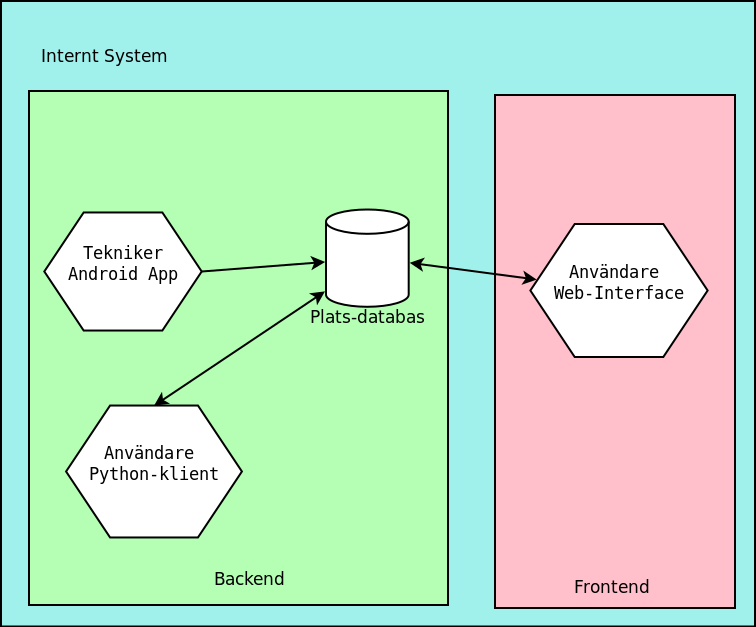
\includegraphics[width=15cm]{media/systemStruktur.png}
 	\caption{Systemstruktur}
 	\label{fig:systemStruktur}
 \end{figure}

 \subsection{Delsystem som kopplar nätverksinformation med en plats}
 Detta delsystem innefattar en Androidapplikation. Den är tänkt att användas av it-tekniker före användning av systemet. Applikationen används för att scanna nätverksinformation i förutbestämda referenspunkter med ett mellanrum på ungefär 2 meter på den aktivitetsbaserade verksamheten. Denna information används senare för att användarenheter ska kunna beräkna sin position i förhållande till dessa referenspunkter. Nätverksinformationen importeras därefter till en databas. När referenspunkterna är inlagda kan nästa delsystem börja användas.

 \subsection{Delsystem som beräknar positionen}
 Detta delsystem innefattar en Python-klient som ska köras i bakgrunden på användardatorn. Python-klientens syfte är att utföra en positionsbestämningsalgoritm med hjälp av den referensdata som finns i databasen och som Androidapplikationen från förra delsystemet har tillhandahållit. När Python-klienten har bestämt positionen för användaren ska den automatiskt lägga in den informationen i databasen kopplat till Python-klientens användaridentitet. Ny bestämning av position utförs var 20e minut. Detta delsystem kommer köras i bakgrunden på en användares dator så att användaren inte aktivt behöver vara involverad i positionsbestämningen.

 \subsection{Delsystem som presenterar position}
 Slutligen består systemet även av ett webb-interface. Detta system använder data som Python-klienten har lagt in i databasen för att i en webbaserad applikation visa positionsinformation om kollegor i verksamheten.

 \subsection{Databasen som håller användare och positionsinformation}
 Databasen är ett delsystem som kommer samspela med alla de andra delsystemen. Den håller information om referenspunkter, användare och deras position.
 Mellan systemet som it-teknikern använder och databasen så måste referenspunktsdata förflyttas manuellt. Då det finns en risk för att referenspunkter kan förstöras om en automatisk uppkoppling utförs bör detta steg göras manuellt. Eftersom inläggningen av referenspunktsdata i databasen sker så pass sällan och endast genomförs genom uppladdning av en .csv-fil innebär den manuella populeringen av databasen inte någon större arbetsbörda. Python-klienten använder sig av SQL-anrop till databasen för att extrahera referenspunkter samt för att lägga in sin position kontinuerligt vid varje körning av algoritmen för positionsbestämning. Webbapplikationen använder även den SQL-anrop till databasen för att erhålla och presentera relevant information.

 %\subsection{Alternativa lösningar}
 % Alternativa lösningar
 % Beskriv strukturen både internt (hur ert eget system är uppbyggt) och externt (vilka andra system ert system kommunicerar med). \textbf{Använd figurer} (och text)!
 % \begin{itemize}
 % \item Vilka delar består systemet av? (T.ex. databas, webbinterface, AI-modul, grafik...) Vilka kommunicerar med vilka, beror av vilka, innehåller vilka andra?
 % \item Vilka delar fanns färdiga att använda/anpassa, vilka utvecklade ni själva? Visa tydligt, gärna grafiskt.
 % \item Finns olika alternativa byggblock eller designval? Vilka är argumenten för/emot valen?
 % \item Hur kommunicerar delarna, vilka protokoll och/eller dataformat används? (Beskriv mer detaljerat i senare, i Huvuddelen.)
 % \item Finns det olika typer av användare/motsv? (T.ex. administratörer resp slut\-an\-vän\-dare?)
 % \end{itemize}
 %
 % \iffalse
 % \subsection{Tänk på följande}
 %
 % Var inte för tekniskt detaljerade här.  Tanken är att ge en översikt över systemet.  Ni behöver inte beskriva objektmetoder etc. i detalj (om de inte är nya och avgörande för resultatet). Tekniska detaljer och implementation beskriver ni snarare i huvuddelen.
 %
 %
 % Se till att ni använder \emph{samma terminologi} i figurer som visar systemet som i texten.
 %
 % Anknyt figurerna till texten på ett tydligt sätt. Om ni t.ex. har separata underrubriker som beskriver olika delar/aspekter av systemstrukturen med tillhörande figur, välj antingen en underrubrik per del i figuren eller använd helt andra underrubriker.  Annars kommer läsaren att undra var underrubriken som beskriver del X är, när det finns underrubriker för alla andra delar.
 % \fi


 \section{Krav och utvärderingsmetoder}\label{krav}

 % Vilka krav ställer ni/andra på ert resultat?
 %
 % hur snabbt? hur många användare? hur strömsnålt? eller vad som är relevant
 % Hur ska ni utvärdera ert arbete/system (så att ni vet om/hur bra ni lyckats)?
 %
 % För de olika funktionaliteterna (och/eller motsv) i ert system, hur ska ni avgöra om de är tillräckligt bra utförda/implementerade? Var går gränsen för ``tillräckligt bra''? (Eller när är de ``för dåliga''?)
 %
 % Skilj på krav och funktionalitet. Själva funktionaliteterna har ni redan beskrivit i systemstrukturen eller huvuddelen nedan. (Har ni krav på saker ni beskriver först i huvuddelen kan ni lägga det här avsnittet efter huvuddelen.)
 %
 % Skriv tydliga krav \emph{som går att utvärdera}.  (Hur snabbt? Hur många användare? Hur strömsnålt? eller vad som är relevant).
 %
 % Beskriv hur utvärderingen ska gå till (automatiserade belastningstester, mätningar, en\-käter, fokusgrupper\ldots).
 % Beskriv hur externa intressenter involveras i utvärderingen.

 Kraven för det här projektet är något som vi tillsammans med Uppsala Kommun kommit fram till. Utöver det som Uppsala Kommun kräver så har vi några generella krav på vår produkt. Det ska vara lättanvänt, robust mot kraschar, hantera känslig information på ett säkert sätt samt bara bestå av välskriven och väldokumenterad kod. Våra egna krav är att systemet i minst 95\% av de totala antalet positioneringar ska lyckas positionera användaren rätt. På grund av tidsbrist kommer endast två typer av tester utföras i en av kommunens byggnader. Dessa två tester kommer bestå av ett våningstest samt ett positioneringstest. Våningstestet utförs genom att analysera den uppskattade positionen för en klientenhet på platser där systemet har integrerats på två våningsplan. Syftet med våningstestet är att analysera om den uppskattade positionen i något fall uppskattas till fel våningsplan. Positioneringstestet utförs genom att en användare rör sig i de lokaler där systemet är integrerat. Användaren sätter sig vid en arbetsplats i en minut och går därefter vidare till nästa arbetsplats. Vid varje arbetsplats utförs en positionsuppskattning. Syftet med positioneringstestet är att undersöka huruvida systemet uppskattar användarens position till samma position som användarens verkliga position.
 Båda dessa tester kommer utvärderas på så sätt att vi för statistik över antalet lyckade positioneringar vid varje körning av positioneringssystemet. Eftersom Uppsala Kommun har en kontorsmiljö uppdelad i arbetsområden av olika storlekar och med olika namn har vi i samråd med dem valt att definiera en lyckad positionsuppskattning som en positionsuppskattning där  positionen uppskattas till namnet för det arbetsområde där användaren befinner sig.
 Statistik om antalet lyckade positioneringar vid dessa tester presenteras i sektion (\ref{resultat}).

 \subsection{Skanningsapplikation för referenspunkter}
 Scanningsapplikationen ska vara ett lättförståeligt och lättanvänt system som ska förenkla förarbetet inför en flytt från kontorsbaserad verksamhet till en aktivitetsbaserad. Detta system kommer enligt intressenten användas av en it-tekniker och måste göras innan någon positionsbestämning kan ske. Vi vill att det ska vara enkelt att använda scanningsapplikationen eftersom det kan vara ett övertygande argument för att använda systemet i sin helhet. Användarvänligheten kommer utvärderas genom att personal från intressenten får gå med och använda applikationen när vi utför övriga tester och därefter ge feedback på användarvänligheten.


 \subsection{Positionsbestämning}
 Uppsala Kommuns vision är att positioneringssystemet ska kunna visa i vilken byggnad, på vilken våning och i vilket område på den våningen som en medarbetare befinner sig. Detta med en felmarginal på max 10 meter. Vi har själva satt upp krav på en felmarginal på max 5 meter eftersom vi tror att det kommer vara möjligt att uppnå. Kraven på exakthet existerar eftersom en godtagbar precision vid positionsbestämningen är en förutsättning för att systemet i sin helhet ska fylla någon funktion. Vi kommer utföra två precisionstester av systemet. Båda testerna kommer utföras i Uppsala Kommuns lokaler på Stationsgatan 12 i Uppsala. Det ena testet gå ut på att testa hur väl systemet kan skilja på olika våningsplan i byggnaden. Det andra testet kommer gå ut på att testa hur väl en användare kan positionsbestämmas till ett specifikt arbetsområde.

 Våningstestet kommer gå till så att referenspunkter utmäts på två olika angränsande våningsplan och läggs in i en databas. Därefter kommer en användare röra sig på de olika våningsplanen samtidigt som programmet för positionsbestämning körs på användarens medhavda dator. För varje positionsbestämning loggas resultatet och användarens verkliga position registreras. Därefter undersöker vi resultaten och ser huruvida systemet kan skilja på olika våningsplan.

 Testet för att undersöka precisionen av positioneringssystemet i relation till ett specifikt område kommer utföras på ett snarlikt sätt som för våningstestet. Skillnaden mot våningstestet kommer vara att referenspunkter kommer utmätas på en hel våning och matchas till respektive område på den våningen. Därefter sker utvärderingen med en logg av resultatet samt registrering av användarens verkliga position på samma sätt som vid våningstestet.

 \subsection{Användarvänlighet i webbapplikationen}\label{krav_anv}
 Kraven på presentationen av medarbetarnas position är att det ska vara enkelt att i webbapplikationen se vart en medarbetare befinner sig. Detta är ett krav som vi bedömer vara viktigt för att kunna demonstrera systemet på ett bra sätt. För intressenten kommer detta inte vara ett prioriterat krav eftersom de vid eventuell lansering planerar att presentera positionsinformationen via en medarbetarportal på deras interna nät. Vi kommer utvärdera denna del av systemet genom att låta en extern person navigera i webbapplikationen och därigenom utvärdera användarvänligheten.

 \section{Implementation av systemet}
 I följande delavsnitt beskrivs implementationen av de olika komponenterna av systemet i mer detalj. Först beskrivs hur applikationen används för att skapa referenspunkter. Sedan beskrivs det hur en position beräknas utifrån dessa punkter. Till sist beskrivs systemets presentationsinterface.

 \subsection{Applikation för scanning vid referenspunkter}
 Målet med applikationen är att kunna populera databasen med referenspunkter som sedan användas i bestämning av en användares position. Detta görs med en mobilapplikation då det är enklare för användarna att gå runt i byggnaden med en mobiltelefon eller surfplatta och skanna av nätverksinformationen istället för med en dator.

 När applikationen startas kommer användaren till en startsida, se figur \ref{fig:mob_main}. Här kan användaren välja att skanna nätverksinformation genom att klicka på ``WIFI SCAN''. Då kommer användaren till en sida där denne kan skanna av nätverksinformation och se 11 accesspunkter, se figur \ref{fig:mob_scan_cal}. På startsidan kan användaren också välja ``ADD REFERENCE POINTS''. När användaren valt ``ADD REFERENCE POINTS'' kommer användaren till en sida där användaren anger ett namn på sin referenspunkt och därefter läggs den till i en lista med referenspunkter , se figur \ref{fig:mob_scan_ref}. Därefter kan användaren klicka på den nyss tillagda referenspunkten för att få upp två alternativ, ``scan this RP'' och ``Delete'', se figur \ref{fig:mob_scan_ref_option}. ``Scan this RP'' betyder att applikationen skannar nätverket för att hitta de tre MAC-adresserna med högst RSSI-värde. Namnet på positionen, de tre MAC-adresserna samt respektive RSSI-värde skapar en referenspunkt. Referenspunkten sparas sedan i en .csv-fil på telefonens interna lagring. CSV, står för comma seperated values och är ett filformat som gör det enkelt att importera fler textrader automatiskt. Detta repeteras tills arbetsområdet har fyllts med lämpligt många referenspunkter, (se sektion \ref{referenspunkter}). Efter det att alla referenspunkter är scannade populeras databasen genom att .csv-filen importeras till databasen manuellt. Valet ``Delete'' tar bort referenspunkten samt alla tillhörande MAC-adresser och RSSI-värden. Slutligen har vi en ``GUIDE'' knapp på startsidan som beskriver föregående information fast i applikationen.

 \begin{figure}[H]
   \centering
   \fbox{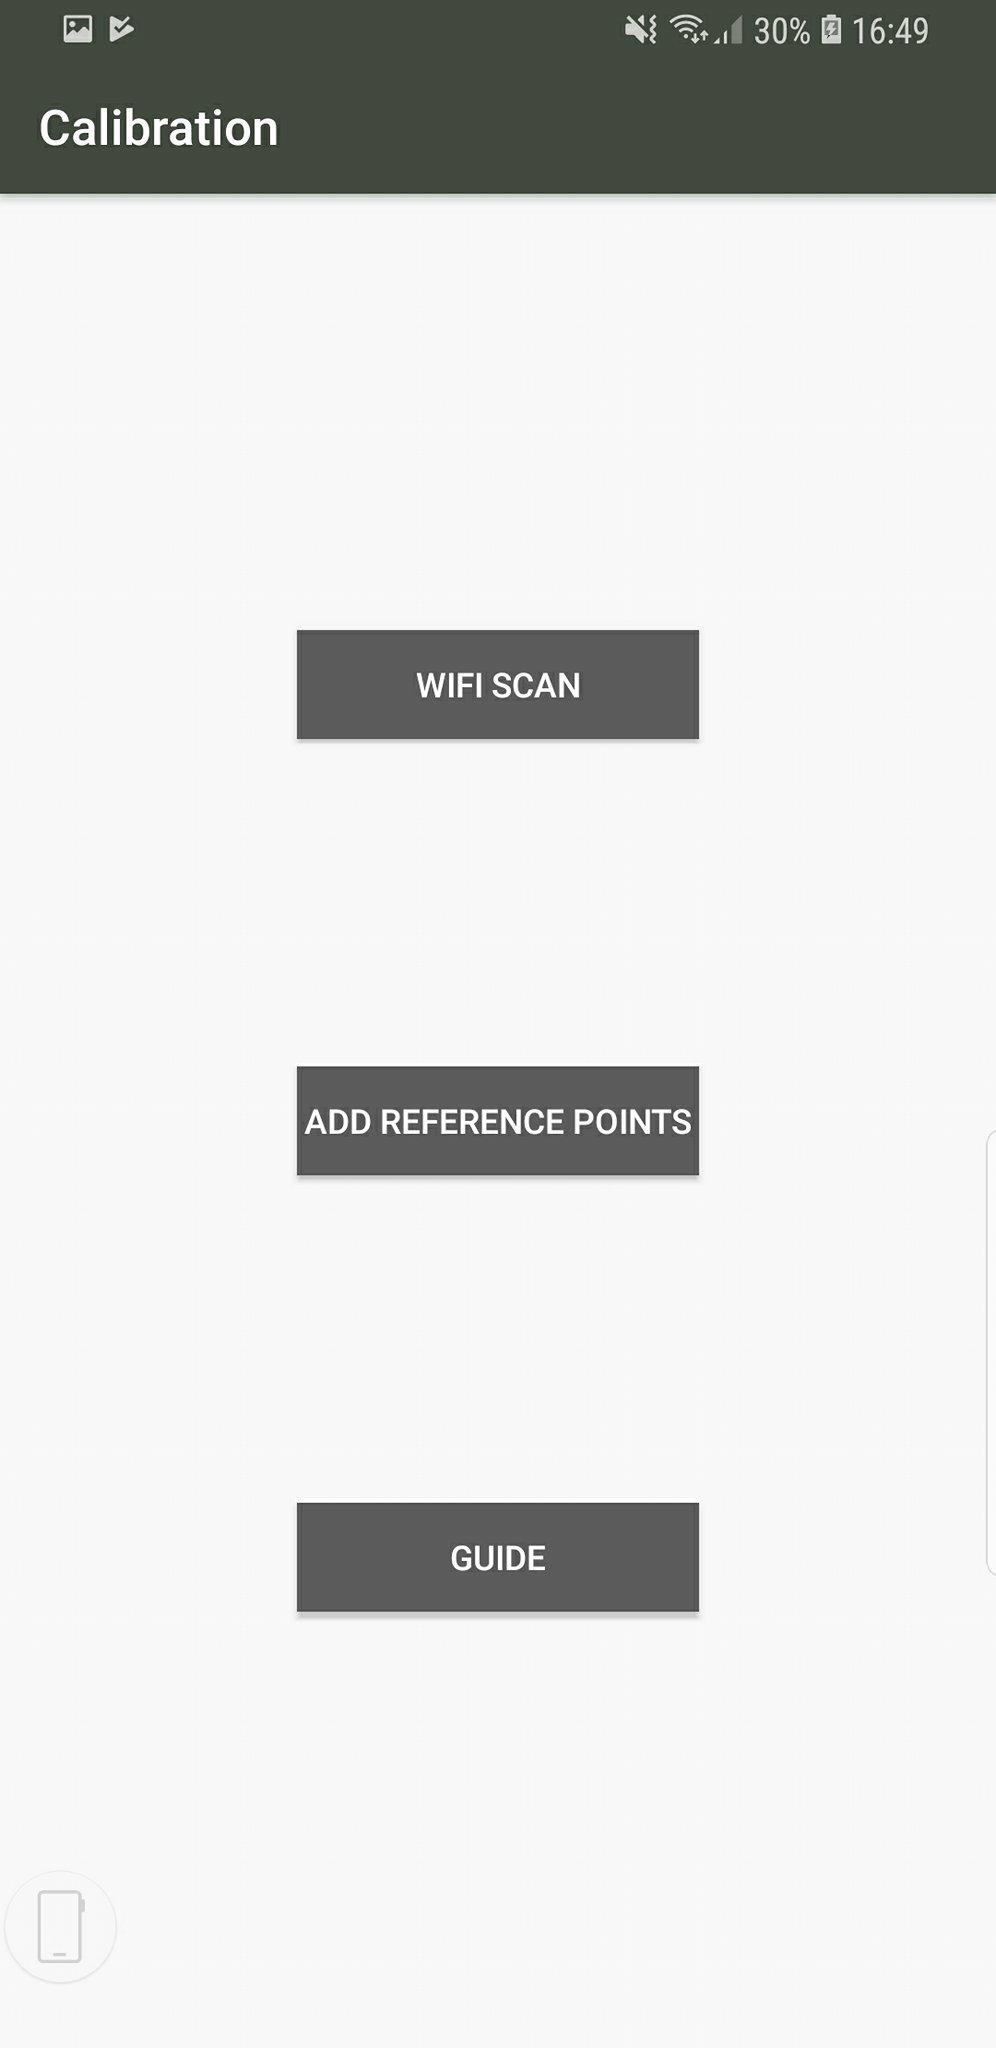
\includegraphics[width=10cm, height=14cm]{media/mob_main.jpg}}
   \caption{En bild på hur startsidan på den mobila applikationen ser ut.}
   \label{fig:mob_main}
 \end{figure}

 \begin{figure}[H]
   \centering
   \fbox{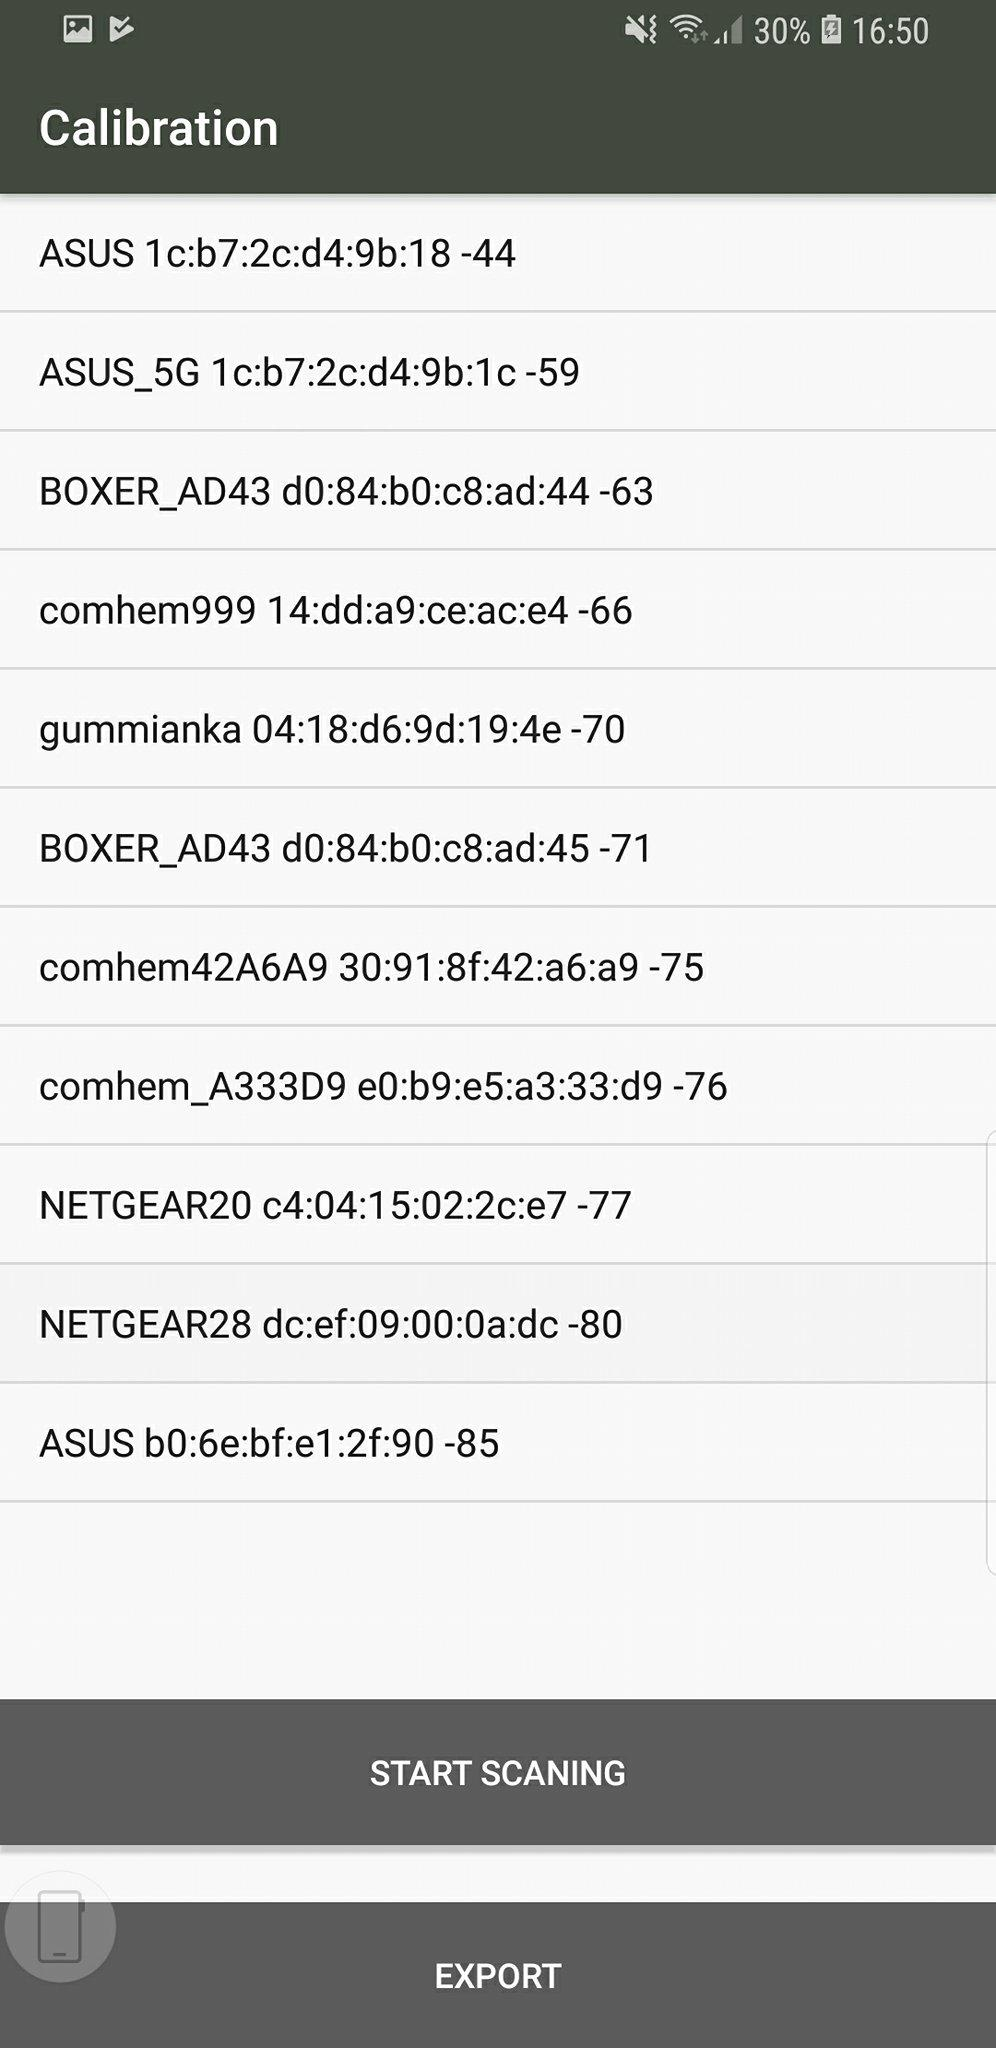
\includegraphics[width=10cm, height=14cm]{media/mob_scan_cal.jpg}}
   \caption{En bild på hur ``WIFI SCAN'' på den mobila applikation ser ut.}
   \label{fig:mob_scan_cal}
 \end{figure}

 \begin{figure}[H]
   \centering
   \fbox{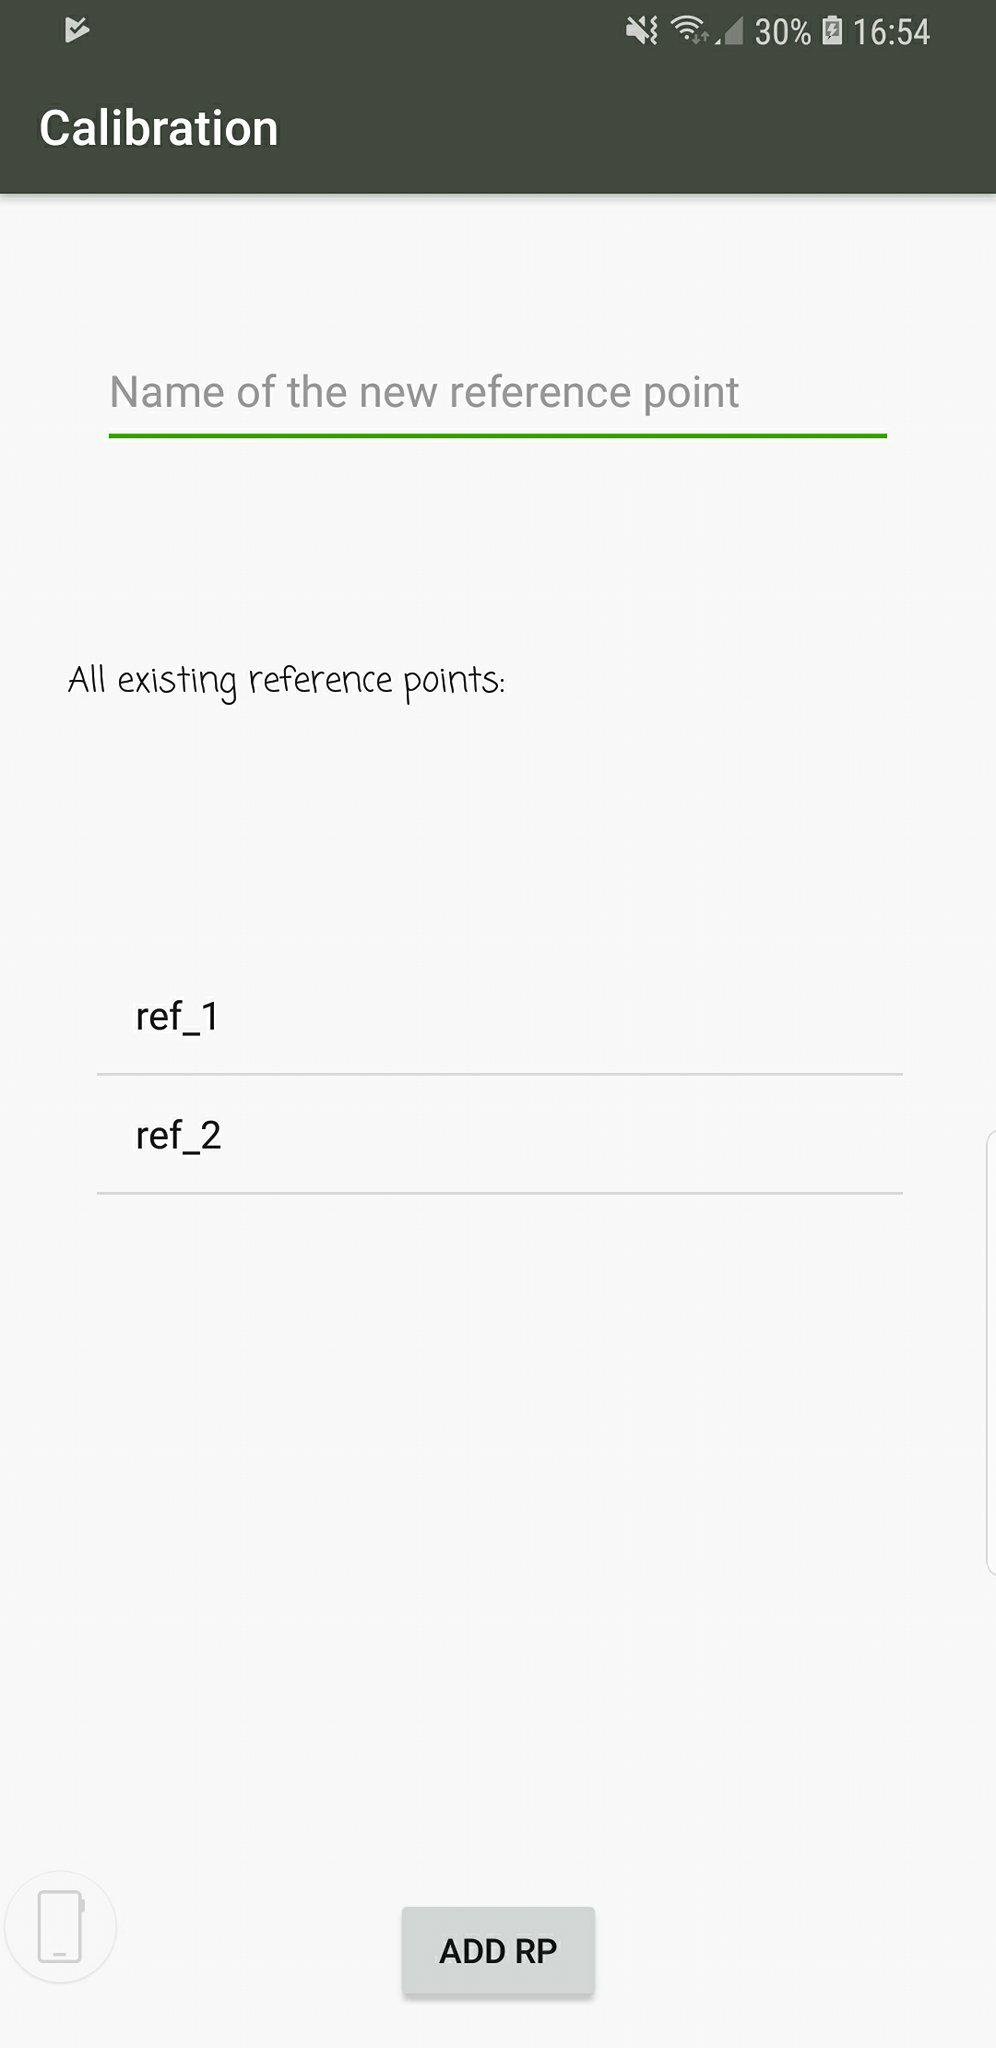
\includegraphics[width=10cm, height=14cm]{media/mob_scan_ref.jpg}}
   \caption{En bild på hur ``ADD REFERENCE POINTS'' på den mobila applikationen ser ut.}
   \label{fig:mob_scan_ref}
 \end{figure}

 \begin{figure}[H]
   \centering
   \fbox{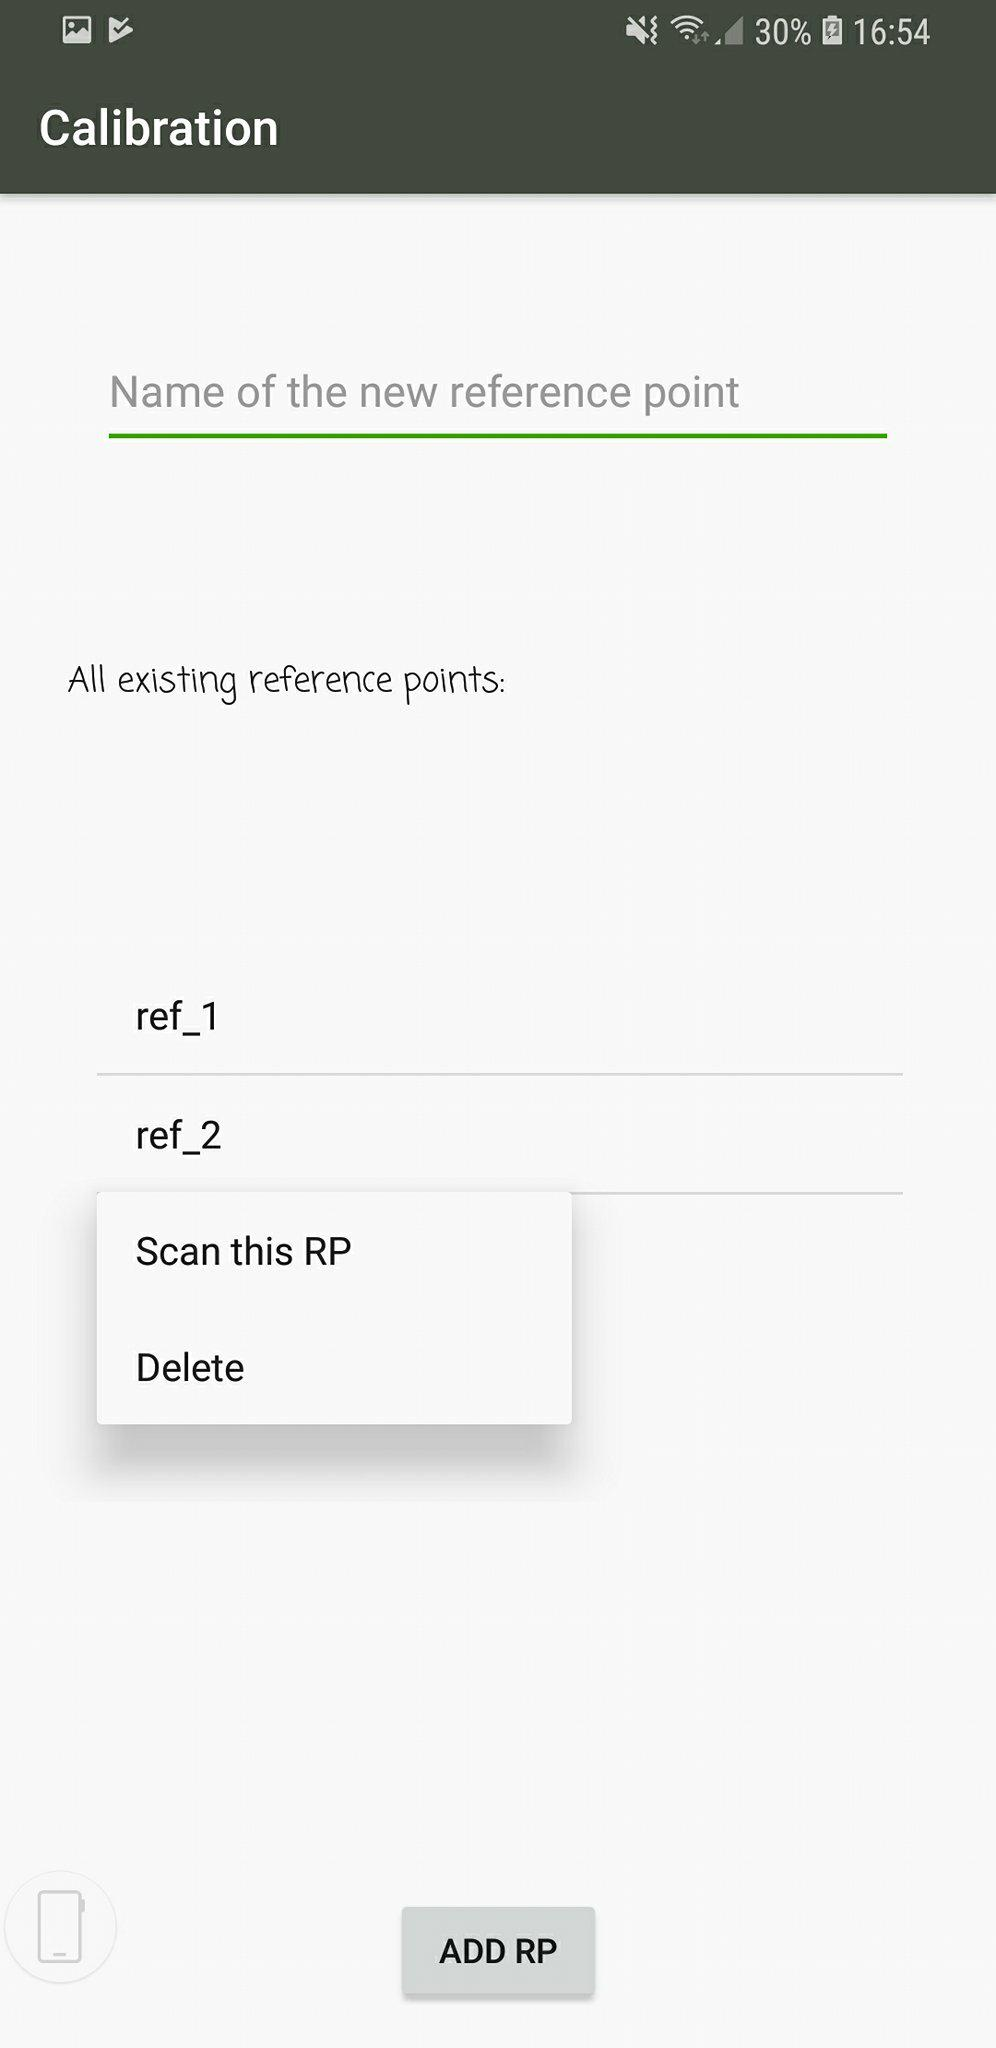
\includegraphics[width=10cm, height=14cm]{media/mob_scan_ref_option.jpg}}
   \caption{En bild på hur valen för en referenspunkt på den mobila applikation ser ut.}
   \label{fig:mob_scan_ref_option}
 \end{figure}

 Fel kan förekomma både vid skanningen samt vid inskrivningen av referenspunkterna till .csv-filen. I båda fallen meddelas användare om detta i form av en ``toast'', vilket är en typ av popup meddelande längst ner på skärmen. När detta förekommer i skanningen behöver användaren skanna om den enskilda positionen som inte fungerade första gången. Detsamma gäller för fel vid inskrivningen till .csv-filen.

 Ytterligare ett fel som kan uppstå är vid importeringen av .csv-filen till databasen. Då databasen inte klarar av å,ä eller ö och inte heller mellanslag i namnet av positionen. Detta fel kan enklast undvikas genom att inte ange namn med dessa bokstäver eller mellanrum. Om det skulle förekomma att användaren råkade skriva in ett å i ett av namnen kan å:et ersättas med ett a eller liknande manuellt i csv filen.%TODO ska sista 2 meningarna vara här eller i avgränsning/future work? JA!

 \subsection{Skript för positionsbestämning}
 Då en klientenhet ska kunna positionsbestämmas behöver klientenheten köra det skript som har utvecklats för positionsbestämning. För att genomföra positionsbestämningen av en klientenhet utför skriptet följande uppgifter:
 \begin{enumerate}
   \item \textbf{Registrerar vilken användare som kör skriptet}
   \item \textbf{Hämtar information om lokalernas referenspunkter från databasen}
   \item \textbf{Utför en scanning av nätverksinformationen}
   \item \textbf{Bestämmer med hjälp av algoritmer positionen för enheten}
   \item \textbf{Uppdaterar databasen med användarens nya position}
 \end{enumerate}

 Nedan redogörs för hur de olika uppgifterna ovan genomförs. %TODO upp och ner ner och upp grisen gal i granens topp, hahaha whaaat?

 \subsubsection{Registrera vilken användare som kör skriptet}
 I den nuvarande versionen av systemet kommer skriptet be användaren om ett användarnamn. Användarnamnet verifieras därefter mot alla registrerade användare som finns i databasen (se sektion \ref{databasen}). Om användarnamnet som användaren anger inte matchar något användarnamn i databasen termineras skriptet. Anledningen är att endast godkända användare ska ha möjlighet att göra skriptet och ladda upp sin positionsinformation i databasen. Användare läggs till av systemadministratören från webbapplikationen (se sektion ~\ref{webbinterface}). I en eventuell senare version av systemet bör skriptet installeras på alla godkända användares enheter och startas så fort användaren loggar in. Då skulle  skriptet kunna läsa av dessa användaruppgifter och köra positionsbestämningen och populeringen av databasen i bakgrunden. Om detta implementeras skulle användandet av systemet kunna ske helt utan interaktion med användaren.

 Denna evenuella och senare funktionalitet anser vi bör vara individuellt utfromad efter en specifik användare av systemet i sin helhet. Därmed nöjer vi oss i vår ``proof of concept'' version att be användaren om ett användarnamn. %TODO ska sista 2 meningarna vara här eller ska de vara i framtida arbete/avgrändningar? JA!

 \subsubsection{Hämta information om referenspunkter från databasen}\label{HamtaInfoDB}
 För att kunna utföra positionsbestämningen behöver klientenheten hämta information om referenspunkterna från databasen. Positionsbestämningen utförs genom vissa beräkningar som vi har valt att genomföra på klientsidan av systemet. Alternativet hade kunnat vara att genomföra alla beräkningar för positionsbestämningen på serversidan av systemet. Om detta hade varit fallet så hade det inte varit nödvändigt att hämta information om referenspunkterna till klienten. Anledningen till valet att utföra beräkningarna på klientsidan var att fördela beräkningsarbetet. Eftersom antalet användare är odefinierat vid en eventuell användning av systemet medför det en osäkerhet om servern klarar av den belastning som förekommer om alla användare ska utföra beräkningar på servern för att bestämma dess position. Eftersom databasen är MySQL-baserad används ett interface för Python som heter PyMySQL\cite{mysqldb}%TODO byt referens
 . PyMySQL erbjuder ett API som ger möjligheten att direkt i pythonkoden skriva funktioner som kan hantera tabeller i databasen. På så sätt hämtas information om referenspunkter och sparar i en temporär lista. %TODO referens

 Nedan följer ett exempel på informationen om en referenspunkt som hämtats från databasen:
 \begin{itemize}
   \item Referenspunkt exempel:
         \newline Område = Polacksbacken, Hus 1, Våning 2, Skrubben.
         \newline MAC 1 = XX:XX:XX:XX:XX:XX
         \newline MAC 2 = YY:YY:YY:YY:YY:YY
         \newline MAC 3 = ZZ:ZZ:ZZ:ZZ:ZZ:ZZ
         \newline RSSI MAC 1 = -45
         \newline RSSI MAC 2 = -48
         \newline RSSI MAC 3 = -50
 \end{itemize}


 Fältet \textit{Området} anger var referenspunkten är utmätt, alltså var nätverksanalysen är genomförd. \\
 \textit{MAC 1}-fältet håller MAC-adressen för den åtkomstpunkt vars RSSI-värde var störst vid nätverksanalysen. Det tillhörande RSSI-värdet ligger i fältet \textit{RSSI MAC 1}\\
  \textit{MAC 2}-fältet håller MAC-adressen för den åtkomstpunkt vars RSSI-värde var näst störst vid nätverksanalysen. Det tillhörande RSSI-värdet ligger i fältet \textit{RSSI MAC 2}\\
   \textit{MAC 3}-fältet håller MAC-adressen för den åtkomstpunkt vars RSSI-värde var tredje störst vid nätverksanalysen. Det tillhörande RSSI-värdet ligger i fältet \textit{RSSI MAC 3}\\


 \subsubsection{Uföra scanning av nätverksinformation} \label{scanning}
 %TODO: SEBBE- här får du gärna bidra lite med din extrema kunskap om exakt hur scanningen går till
 Då en klientenhet ska positionsbestämmas kör skriptet en scanning för att se vilken trådlös nätverksinformation som kan upptäckas. Den information som sparas vid scanningen är tillgängliga åtkomstpunkter samt tillhörande RSSI-värde (se sektion \ref{RSSI}). Vid den scanningen läses upp till 10 stycken tillgängliga åtkomstpunkter in och sorteras med avseende på vilken åtkomstpunkt som har högst RSSI-värde. Ett exempel på resultatet efter scanningen ser ut som föjler:

   \begin{itemize}
   \item Klientenhetsscanning exempel:
         \newline MAC 1 = AA:AA:AA:AA:AA:AA,  RSSI = -20
         \newline MAC 2 = BB:BB:BB:BB:BB:BB,  RSSI = -25
         \newline MAC 3 = CC:CC:CC:CC:CC:CC,  RSSI = -30
         \newline MAC 4 = DD:DD:DD:DD:DD:DD,  RSSI = -35
         \newline MAC 5 = EE:EE:EE:EE:EE:EE,  RSSI = -40
         \newline MAC 6 = FF:FF:FF:FF:FF:FF,  RSSI = -45
         \newline MAC 7 = GG:GG:GG:GG:GG:GG,  RSSI = -50
         \newline MAC 8 = HH:HH:HH:HH:HH:HH,  RSSI = -55
         \newline MAC 9 = II:II:II:II:II:II,  RSSI = -60
         \newline MAC 10 = JJ:JJ:JJ:JJ:JJ:JJ,  RSSI = -65
   \end{itemize}

 \subsubsection{Algoritmer för positionsbestämmning}\label{algoritm}
 För att utföra positionsbestämningen av klientenheten körs en algoritm i skriptet. Den algoritm som valdes för positionsbestämning är en variant av KNN (se sektion \ref{KNN}). Vid algoritmer av typer KNN analyseras ett antal (K) Nearest Neigbours (NN). Eftersom informationen om tre åtkomstpunkter för varje sparad referenspunkt finns tillgänglig analyseras de tre närmaste grannarna.
 Målet med algoritmen är att avgöra vilken sparad referenspunkt som befinner sig närmast klientenhetens fysiska position. Då algoritmen för att positionsbestämma en klientenhet körs kommer resultatet bli samma position som positionen för den bäst matchande referenspunkten. För att åstadkomma detta har två typer av positionsbestämningsmetoder använts. Dessa två beskrivs nedan.

 \paragraph{Metod 1 - Närliggande åtkomstpunkter}
 \leavevmode\\
 Metod 1 bygger på teorin att de referenspunkter som innehåller åtkomstpunkter som överensstämmer med åtkomstpunkterna med högst RSSI-värde i klientenhetens lista (se exempel i sektion \ref{scanning}) är de referenspunkter som befinner sig närmast klientenheten. Om det går att finna en referenspunkt vars tre åtkomstpunkter återfinns som topp tre åtkomstpunkter i klientenhetens lista bör denna referenspunkt befinna sig i nära anslutning till klientenheten.
 Metod 1:s syfte är alltså att finna referenspunkter som har samma närmast intilliggande åtkomstpunkter som klientenheten.

 Algoritmen för metod 1, med syfte att uppskatta vilken referenspunkt som befinner sig närmast klientenheten ser ut på följande sätt:

   \begin{itemize}
     \item \textbf{Steg 1}
     \newline
     Analysera alla tillgängliga referenspunkter i databasen och sortera ut alla som har minst en åtkomstpunkt som överensstämmer med en åtkomstpunkt i listan hos klientenheten. Alla referenspunkter som har en överensstämmande åtkomstpunkt sparas för vidare beräkningar. Om ingen referenspunkt har en tillhörande åtkomstpunkt som återfinns i klientenhetens lista med åtkomstpunkter är inte positionsbestämning möjligt och resultatet blir ``position okänd''.
     Detta steg görs för att slippa utföra mer krävande beräkningar på alla referenspunkter i databasen.
     \item \textbf{Steg 2}
     \newline
     Utifrån de referenspunkter som sorterats fram från steg 1 görs en ny sortering. Nu undersöks vilket det högsta antalet matchande åtkomstpunkter är hos en referenspunkt. Det högsta möjliga antalet matchande åtkomstpunkter är 3 eftersom det finns 3 åtkomstpunkter lagrade för varje referenspunkt. Alla de referenspunkter som har samma högsta antal matchande referenspunkter sorteras ut och sparas.
     Om det till exempel finns fyra referenspunkter vars alla tillhörande åtkomstpunkter finns med i klientenhetens lista sparas dessa fyra referenspunkter för vidare beräkningar. Syftet med detta steg är det samma som syftet i steg 1.

     \item \textbf{Steg 3}
     \newline
     I steg 3 ges alla kvarvarande referenspunkter poäng baserat på hur väl ordningen i de åtkomstpunkter som finns lagrade för referenspunkten överensstämmer med ordningen för åtkomstpunkterna som är scannade av klientenheten. Eftersom både referenspunkternas och klientenhetens åtkomstpunkter är sorterade baserat på RSSI-värdet (signalstyrkan) kan poängsystemet användas för att avgöra vilken referenspunkt som troligtvis är den som befinner sig närmast klientenheten.
     Högsta möjliga poäng tilldelas en referenspunkt vars 3 lagrade åtkomstpunkter återfinns bland de tre åtkomstpunkerna med bäst signalstyrka hos klientenheten samt med samma inbördes ordning. Varje åtkomstpunkt hos referenspunkten jämförs med varje åtkomstpunkt i klientenhetens lista. Ju högre upp i listan åtkomstpunkten befinner sig, både i referenspunkten och i klientlistan, ju högra poäng tilldelas referenspunkten. När varje åtkomstpunkt i referenslistan jämförts läggs poängen för varje åtkomstpunkt ihop och ger referenspunktens slutgiltiga poäng.
     Den referenspunkt som fått högst totalpoäng bedöms vara den referenspunkt som befinner sig närmast klientenheten varvid klientenhetens position bestäms till samma position som för den vinnande referenspunkten.
     En illustration av poängutdelningsprocessen ges i figurerna \ref{fig:MAC1},\ref{fig:MAC2},\ref{fig:MAC3} nedan.
     MAC-adresserna är åtkomstpunkternas unika namn.

   \begin{figure}[H]
     \centering
   	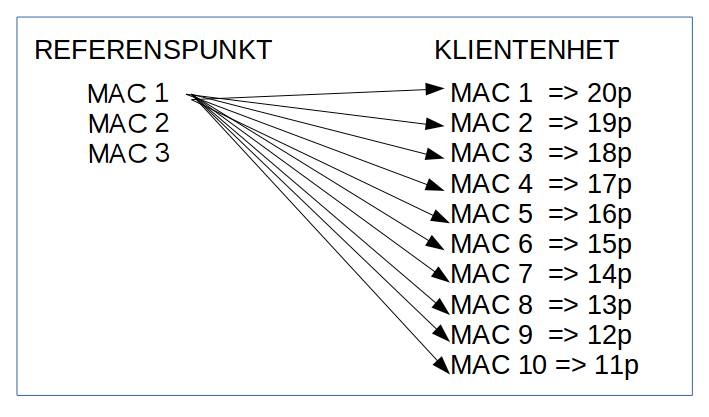
\includegraphics[width=10cm]{media/MAC_1.png}
   	\caption{Poängsystem för åtkomstpunkt 1}
   	\label{fig:MAC1}
   \end{figure}
   \begin{figure}[H]
     \centering
   	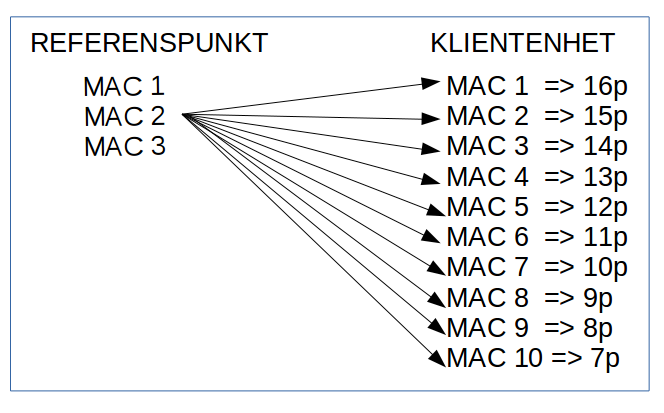
\includegraphics[width=10cm]{media/MAC_2.png}
   	\caption{Poängsystem för åtkomstpunkt 2}
   	\label{fig:MAC2}
   \end{figure}
   \begin{figure}[H]
     \centering
   	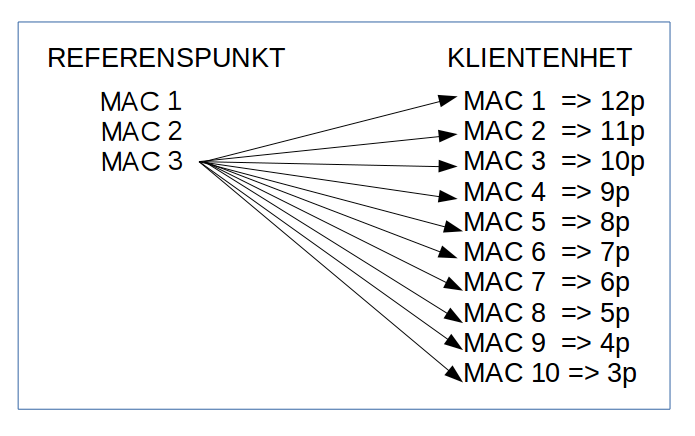
\includegraphics[width=10cm]{media/MAC_3.png}
   	\caption{Poängsystem för åtkomstpunkt 3}
   	\label{fig:MAC3}
   \end{figure}
 %TODO Till och med jag har lite svårt att förstå dina bilder. Alla klienenheter har ju samma macaddress som referenspunkten. Är det en typo eller har det med RSSI att göra? om det har med RSSI bör man nog visa det också! Kommentar - Står väl i texten innan?
   \item \textbf{Steg 4}
   \newline
   Om fler än en referenspunkt slutar på samma poäng i steg 3 av algoritmen betyder det att det inte endast med hjälp av att undersöka den inbördes ordningen för åtkomstpunkterna kan avgöras vilken som teoretiskt sett bör vara den som bäst överensstämmer med klientenhetens position. Vid de fall som detta uppstår vill vi ändå kunna utse en referenspunkt som den bäst matchande. Det gör vi genom att övergå till Metod 2 för positionsbestämning.
 \end{itemize}
 %TODO väldigt lång förstamening i steg 4. Sant

 \paragraph{Metod 2 - Analys av RSSI-värden}
 \leavevmode\newline
 I de fall som Metod 1 för positionsbestämningen av en klientenhet inte har lyckats avgöra vilken referenspunkt som bäst matchar klientenhetens position behöver vi ytterligare en metod. Metoden används för att utse \textbf{en} specifik referenspunkt som klientenhetens position bäst matchar. Om Metod 1 inte kunnat fastställa en specifik referenspunkt betyder det att två eller fler kandiderar om att vara bäst matchande. Dessa kandidater skickas vidare till Metod 2.

 Metod 2 har till uppgift att analysera RSSI-värdet för varje åtkomstpunkt som återfinns i både referenspunktens och klientenhetens lista med åtkomstpunkter.
 Teorin som Metod 2 bygger på är att ju mindre RSSI-värdet skiljer sig åt för åtkomstpunkten till klientenhet respektive åtkomstpunkten till referenspunkt desto troligare är det att avståndet mellan åtkomstpunkt och klientenhet respektive åtkomstpunkt och referenspunkt är detsamma. Teorin illustreras i figur \ref{fig:TEO2} nedan.

 \begin{figure}[H]
   \centering
   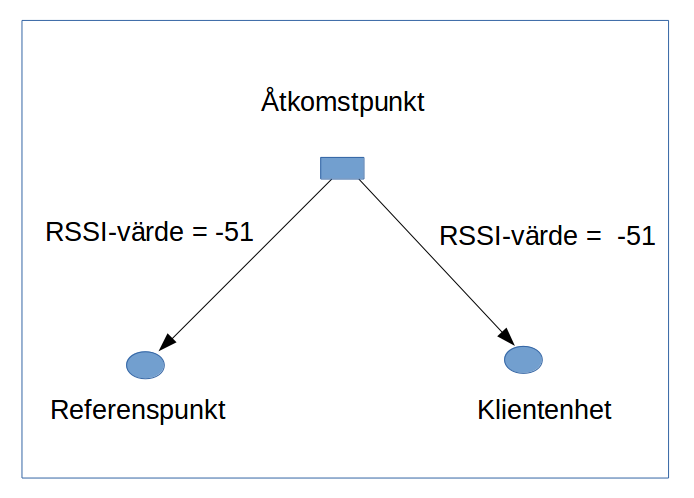
\includegraphics[width=10cm]{media/TeoriMetod2.png}
   \caption{Illustration av teorin bakom Metod 2 för positionsbestämning}
   \label{fig:TEO2}
 \end{figure}
 %TODO man kan kanske ha en till punkt i bilden för att visa att referenspunkten och klienenheten är närmare varandra än den punkt som har ett annat RSSI värde. Nu ser det ut som om trots att de har samma RSSI värde så är de inte nära varandra.

 Teorin bakom Metod 2 bygger därmed på att om klientenheten och en referenspunkt har ett RSSI-värde till samma åtkomspunkt som överensstämmer så bör de även befinna sig på samma avstånd från åtkomstpunkten. Detta gäller tyvärr till viss del bara i teorin eftersom signalen från åtkomstpunkten kan reflekteras mot väggar, tak och annat möblemang vilket påverkar RSSI-värdet\cite{zanca2008experimental}. Ett annat problem som gör denna teori mindre tillförlitlig i praktiken är enligt Lui m. fl. att olika hårdvara för trådlös nätverksmottagning kan ge olika RSSI-värden trots identiska förhållanden\cite{problem_with_RSSI}. Dessa problem är anledningen till att vi väljer att implementera Metod 2, som är baserad på denna teori, som ett eventuellt sista steg i positionsbestämningen.

 Algoritmen för Metod 2 som är baserad på teorin beskriven ovan har vi konstruerat som följer.

 \begin{enumerate}
   \item Differensen i RSSI-värde för klientenheten samt för en referenspunkt till samma åtkomstpunkt beräknas och sparas. Detta görs för varje överensstämmande åtkommspunkt hos en referenspunkt och klientenheten.
   \item Differenserna i RSSI-värde för varje överensstämmande åtkomstpunkt adderas. Detta gör att varje referenspunkt får ett sammanlagt värde på differenserna uppmätta i steg 1.
   \item Den referenspunkt med lägst sammanlagd differens uppskattas till att vara den referenspunkt som befinner sig närmast klientenheten.
 \end{enumerate}


 Figur \ref{fig:MET2} ger är ett exempel på en situation när Metod 2 används och hur positionsbestämningen går till. Observera att den åtkomstpunkt med högst RSSI-värde i klientenhetens list även är den åtkomstpunkt i båda referenspunkternas lista som har högst RSSI-värde. Observera även att det samma gäller för åtkomstpunkten med näst högst RSSI-värde. Det är viktigt att dessa observationer påpekas då det endast är i dessa fall som Metod 2 används.

 \begin{figure}[H]
   \centering
   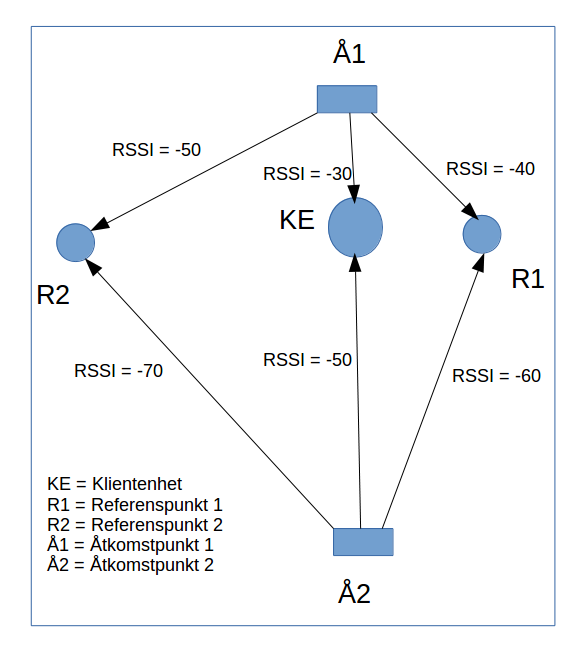
\includegraphics[width=10cm]{media/MET2.png}
   \caption{Exempel på när användning av Metod kan förekomma}
   \label{fig:MET2}
 \end{figure}

 Det som sker i figur \ref{fig:MET2} är att både referenspunkt 1, referenspunkt 2 och klientenheten har åtkomstpunkt 1 som den åtkomstpunkt vars RSSI-värde är lägst. Både referenspunkt 1, referenspunkt 2 och klientenheten har även gemensamt att åtkomstpunkt 2 är den åtkomstpunkt vars uppmätta RSSI-värde är näst högst. Då antas det att både referenspunkt 1 och referenspunkt 2:s tredje registrerade åtkomstpunkt inte finns med i klientenhetens lista över åtkomstpunkter. Beräkningarna som följer ser då ut på följande sätt.

 Först jämförs RSSI-värdena för klientenheten och referenspunkt 1 i förhållande till åtkomstpunkterna 1 och 2.

 Först mot åtkomstpunkt 1: $$ RSSI (KE,\verb|Å|1)  -  RSSI (R1,\verb|Å|1) = -30 - (- 40) = 10 $$

 Sedan mot åtkomstpunkt 2: $$ RSSI (KE,\verb|Å|2)  -  RSSI (R1,\verb|Å|2) = -50 - (- 60) = 10 $$

 Därefter adderas resultaten för analysen av referenspunkt1: $$ 10 + 10 = 20$$

 Därefter jämförs RSSI-värdena för klientenheten och referenspunkt 2 i förhållande till åtkomstpunkterna 1 och 2.

 Först mot åtkomstpunkt 1: $$ RSSI (KE,\verb|Å|1)  -  RSSI (R2,\verb|Å|1) = -30 - (- 50) = 20 $$

 Sedan mot åtkomstpunkt 2: $$ RSSI (KE,\verb|Å|2)  -  RSSI (R2,\verb|Å|2) = -50 - (- 70) = 20 $$

 Därefter adderas resultaten för analysen av referenspunkt2: $$ 20 + 20 = 40$$

 Det resulterar i att referenspunkt 1 genererar ett lägre slutvärde än referenspunkt 2. Därmed antas referenspunkt 1 befinna sig närmare klientenheten och klientenhetens position uppskattas till samma position som för referenspunkt 1.

 \subsubsection{Uppdatera databasen med klientenhetens position}
 Efter det att klientenhetens position är bestämd är det sista som sker i skriptet att databasen uppdateras med användarens nya position. Detta görs med hjälp av samma API som vi får tillgång till genom användandet av PyMySQL (se sektion \ref{HamtaInfoDB}).

 \subsection{Databasens uppbyggnad}\label{databasen}
 Databasen är hjärtat och den enda resursen som egentligen behöver delas mellan alla enheter i systemet. Den håller data om referenspunkter samt data om användare samt deras position. Varje delsystem som konstruerats gör anrop till databasen. Skanningsapplikationen producerar referenspunkter som läggs in i en tabell. Skriptet för positionsbestämning kontrollerar att användaren är en befintlig användare och lägger sedan in vilken position användaren har. Insättningen sätts in i de relationella tabellerna som håller vilken position varje användare har, och har haft. Webbapplikationen som ska presentera datan på ett tydligt sätt går in och hämtar varje användare, länkar dessa med vilken position och presenterar detta.

 \subsubsection{Tabell för referenspunkter}
 Tabellen för referenspunkterna har konstruerats manuellt med SQL direkt in i databasen, se figur ~\ref{fig:db_tabeller}.
 Den är konstruerad som en enskild tabell. Anledningen till att vi endast använder en enskild tabell i det här fallet är för att det underlättar importeringen av .csv-filen från scanningsapplikationen. Tabellens struktur ser ut som följer.

 \begin{itemize}
   \item id - som bara autinkrementeras, ingen speciell funktion.
   \item position - positionen som referenspunkten ska innebära.
   \item address1 - MAC-adressen för den starkaste accesspunkten sorterat enligt RSSI.
   \item address2 - MAC-adressen för den näst starkaste accesspunkten sorterat enligt RSSI.
   \item address3 - MAC-adressen för den tredje starkaste accesspunkten sorterat enligt RSSI.
   \item rssi1 - RSSI för den starkaste accesspunkten sorterat enligt RSSI.
   \item rssi2 - RSSI för den näst starkaste accesspunkten sorterat enligt RSSI.
   \item rssi3 - RSSI för den tredje starkaste accesspunkten sorterat enligt RSSI.
 \end{itemize}
 %TODO ska det vara stora bokstäver i början av varje item?

 \subsubsection{Relationella tabeller för användare och deras position}
 Databasen innehåller även två tabeller som
 kopplas ihop med hjälp av Foreign Keys respektive Primary Keys och håller användare och deras position, se figur ~\ref{fig:db_tabeller}.
 Dessa två tabeller konstrueras av Django (se sektion \ref{django}), webbapplikations-ramverket som används, när modeller definieras i webbapplikationen. Att definiera modeller är ett objektorienterat sätt att skapa tabeller på. En modell skapas, sedan definieras vilka fält modellen ska ha på enskilda rader och sedan översätter Django detta till SQL-kod samt migrerar det till databasen.

 Tabellen som håller användarinformation är strukturerad enligt följande
 \begin{itemize}
   \item  u\_id - Primary Key som länkar till tabellen för användares position %TODO vet man vad primary key är?
   \item  u\_username - användarens användarnamn
   \item  u\_fullname - användarens för- och efternamn
   \item  u\_show\_position - huruvida användaren vill visa sin position
 \end{itemize}

 Tabellen som håller en användares position är strukturerad enligt följande
 \begin{itemize}
   \item u\_id - Foreign Key som länkar till tabellen för användarinformation
   \item u\_position - Användarens position
   \item u\_datetime - Datum och tid som användarens position lades in i tabellen
 \end{itemize}

 \begin{figure}[H]
   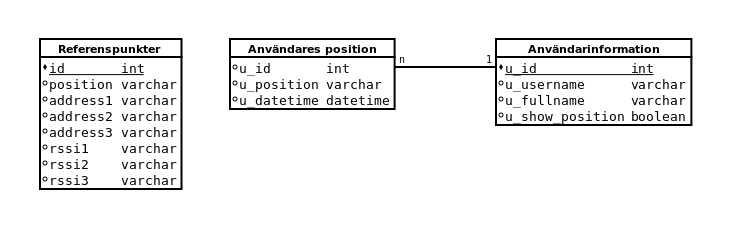
\includegraphics[width=15cm]{media/db_tabeller.png}
   \caption{Tabeller i databasen}
   \label{fig:db_tabeller}
 \end{figure}

 \subsection{Webbapplikation för presentation av användares position} \label{webbinterface}
 Webbapplikationen är byggd i webbapplikationsramverket Django samt Materialize %TODO VAd är?
 för att snabbt och enkelt göra webbapplikationen responsiv och designad. %TODO referens
 Med django kommer automatiskt en webbserver som kan startas lokalt på en användares dator. I implementationen kan servern köras både lokalt eller delat. Att webbserver körs lokalt drabbar inte funktionaliteten i systemet eftersom det enda som behöver vara delat mellan alla användare är databasen.

 Webbapplikationen utgörs initialt av en inloggningssida (se figur \ref{fig:comp_log_in}) där användaren på arbetsplatsen måste logga in för att se positioner för andra användare. Användare kan även registrera ett konto, se figur \ref{fig:comp_sign_in}. När användaren har loggat in så har denne möjlighet att se andra användares position, söka efter specifika användare samt välja att dölja sin position, se \ref{fig:comp_search} . I den föregående figuren såg vi att alla förutom Nils Wik valde att visa sin position. Om en användare inte är inloggad kommer endast en text visas, se figur \ref{fig:comp_not_logged_in}.

 \begin{figure}[H]
   \centering
   \fbox{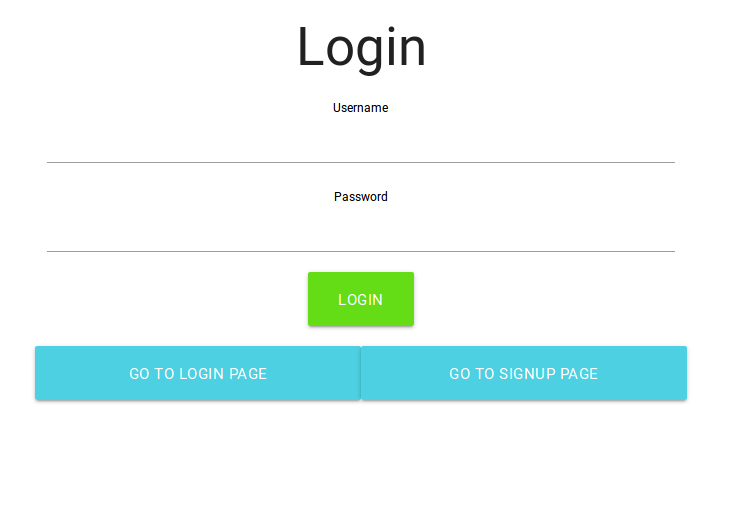
\includegraphics[width=10cm, height=12cm]{media/comp_log_in.png}}
   \caption{En bild på hur inloggning till webbapplikationen ser ut ifrån en dator.}
   \label{fig:comp_log_in}
 \end{figure}

 \begin{figure}[H]
   \centering
   \fbox{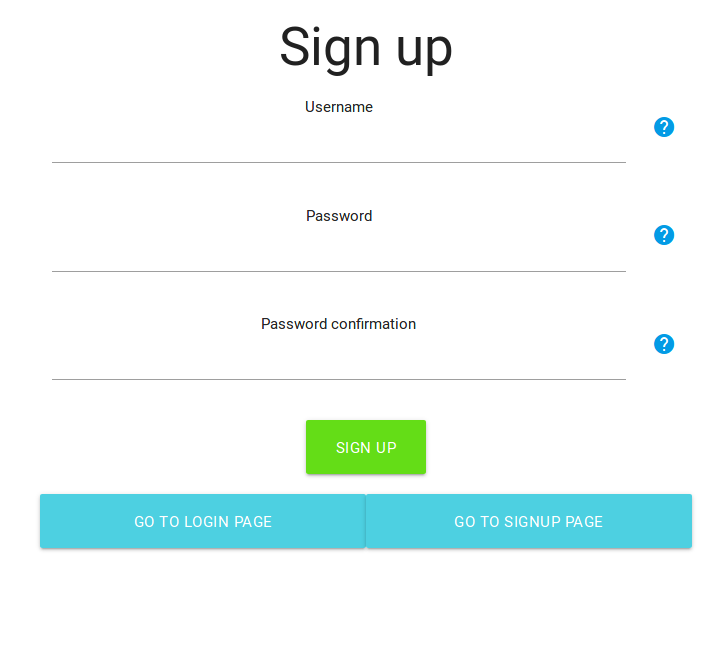
\includegraphics[width=10cm, height=12cm]{media/comp_sign_in.png}}
   \caption{En bild på hur registrering till webbapplikationen ser ut ifrån en dator.}
   \label{fig:comp_sign_in}
 \end{figure}

 \begin{figure}[H]
   \centering
   \fbox{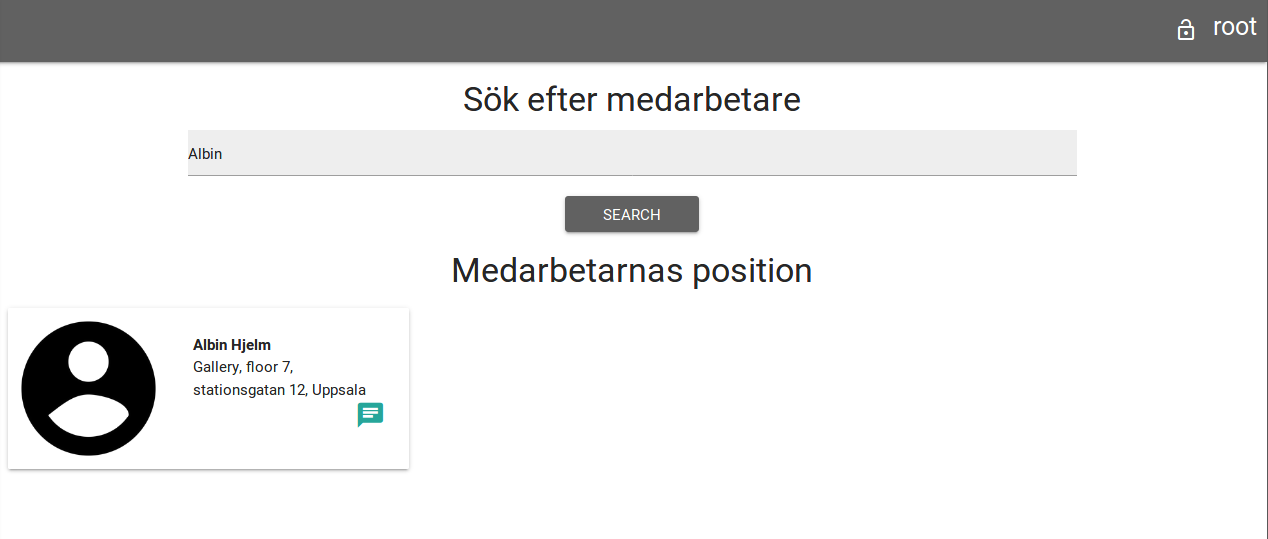
\includegraphics[width=14cm, height=10cm]{media/comp_search.png}}
   \caption{En bild på en sökninga av en medarbetare ifrån en dator.}
   \label{fig:comp_search}
 \end{figure}
 \leavevmode

 \begin{figure}[H]
   \centering
   \fbox{
\includegraphics[width=14cm]{media/comp_not_logged_in.png}}
   \caption{En bild på en icke inloggad användares vy ifrån en dator.}
   \label{fig:comp_not_logged_in}
 \end{figure}

 Webbapplikationen erbjuder även en administrativ hemsida. För att få tillgång till denna hemsida måste användaren ha särskild behörighet. Skaparen av hemsidan har behörighet och kan i sin tur kan dela med sig av behörigheten till andra användare. I den administrativa hemsidan kan administratören se alla användare, ge behörigheter till olika andra användare (bland annat behörigheten till att se den administrativa hemsidan) och alternativt även ändra i den administrativ hemsidan.

 Webbapplikationen är även tillgänglig från mobila enheter. Inloggning och registrerings-hemsidan presenteras i figur \ref{fig:mob_login} samt \ref{fig:mob_sign_up}. Efter att användaren har loggat in kommer denne till hemsidan för sökning av andra användare, positionsvisning mm. Hemsidans vy från en mobiltelefon presenteras i figur \ref{fig:mob_show_position}.

 \begin{figure}[H]
   \centering
   \fbox{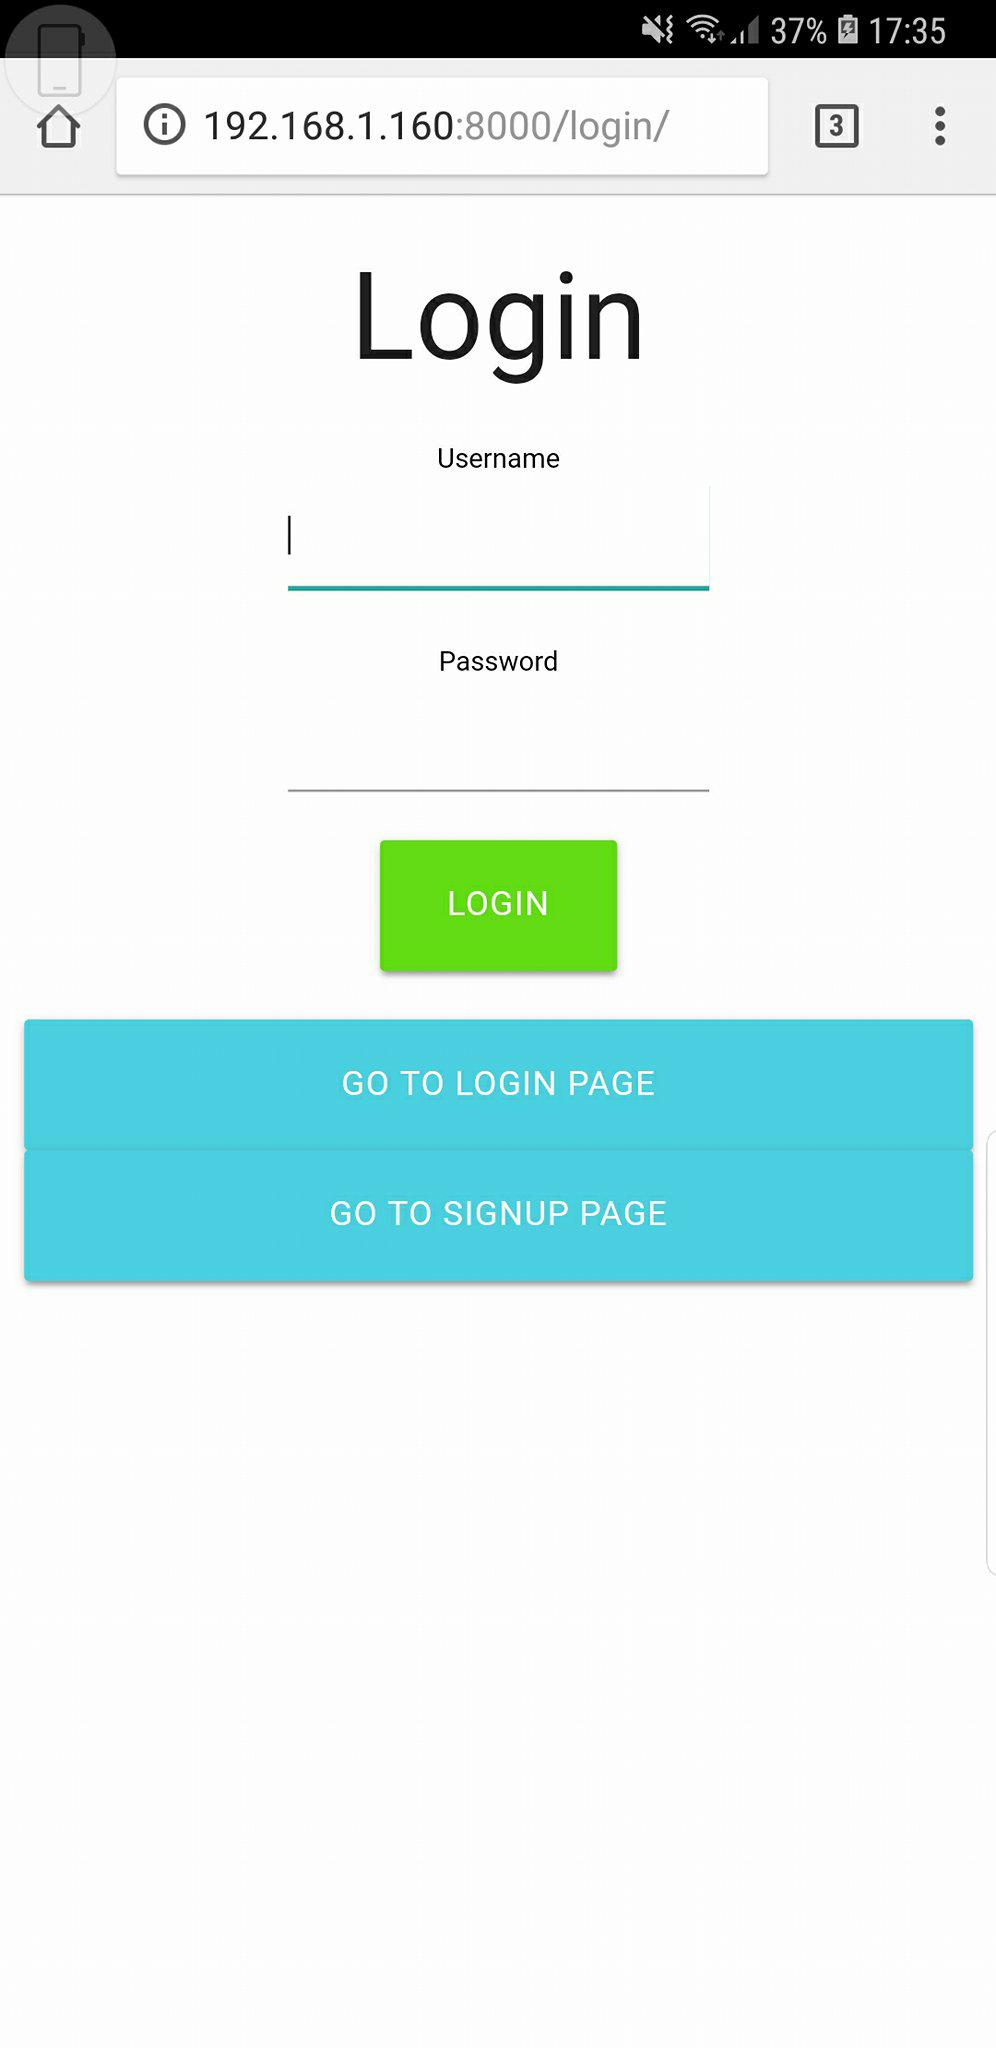
\includegraphics[width=10cm, height=14cm]{media/mob_login.jpg}}
   \caption{Hur inloggning till webbapplikationen ser ut ifrån en mobiltelefon.}
   \label{fig:mob_login}
 \end{figure}

 \begin{figure}[H]
   \centering
   \fbox{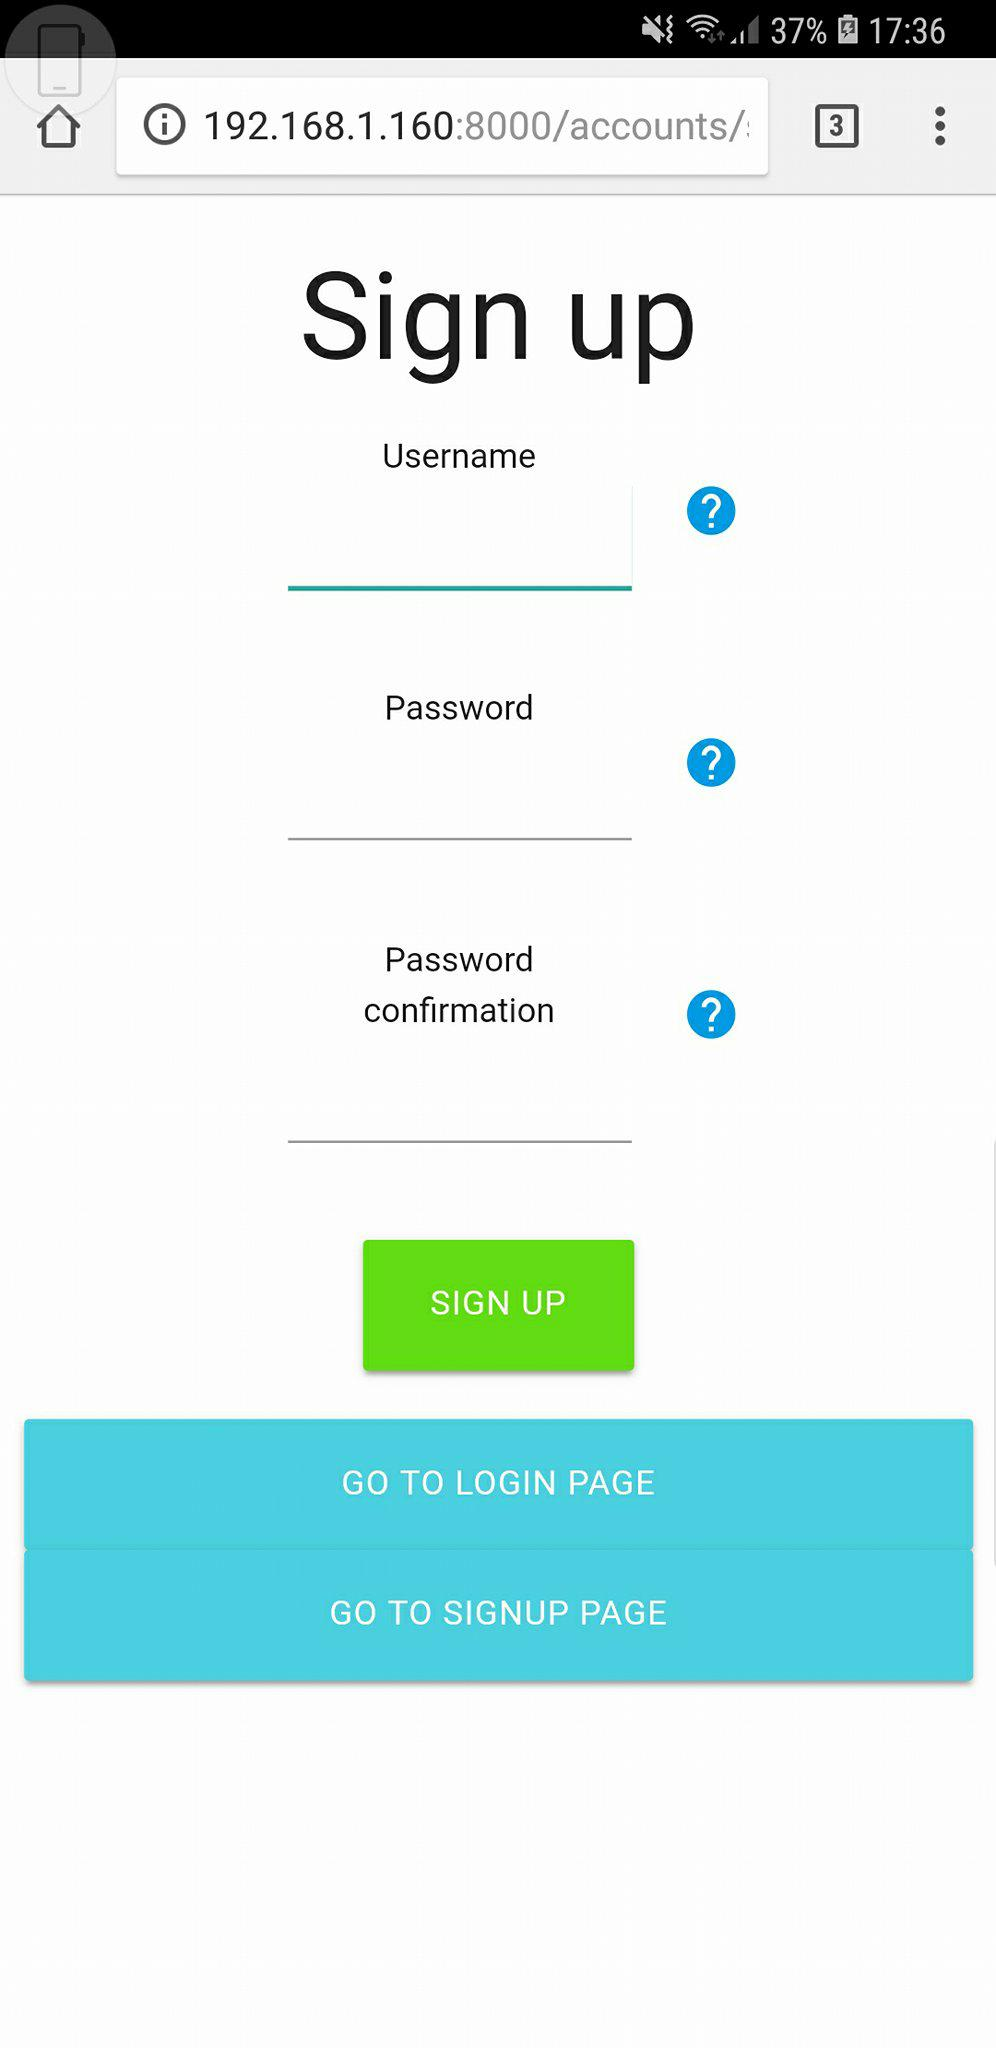
\includegraphics[width=10cm, height=14cm]{media/mob_sign_up.jpg}}
   \caption{Hur registrering till webbapplikationen ser ut ifrån en mobiltelefon.}
   \label{fig:mob_sign_up}
 \end{figure}

 \begin{figure}[H]
   \centering
   \fbox{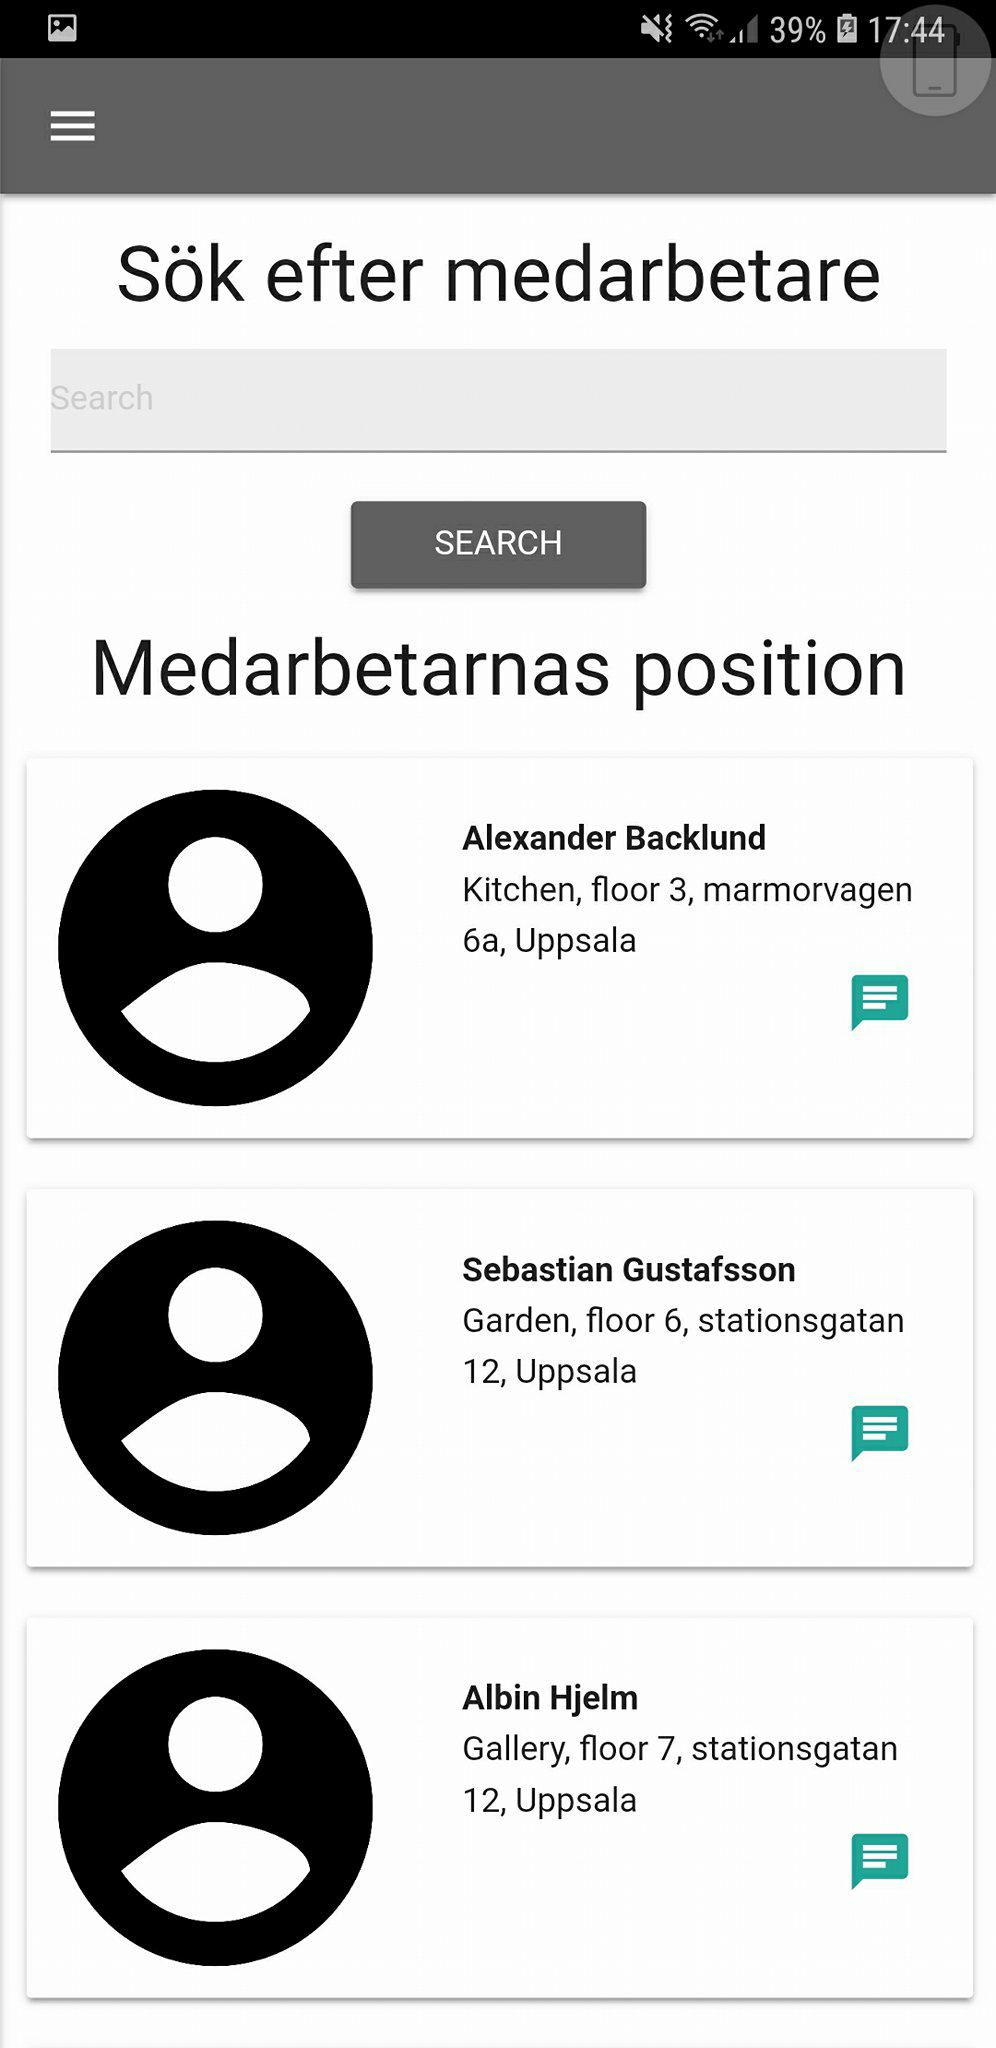
\includegraphics[width=10cm, height=14cm]{media/mob_show_position.jpg}}
   \caption{Bild på en inloggad användares vy ifrån en mobiltelefon.}
   \label{fig:mob_show_position}
 \end{figure}


 \iffalse
 \section{DEL x}\label{sec:delX}
 Mellan introduktion och avslutning finns ett eller sannolikt \emph{flera} avsnitt (``huvuddelen'') som innehåller själva bidraget.  Ni får själva välja passande rubriker (INTE ``Huvuddel'' eller ``Bidrag'').  Rubrikerna i huvuddelen ska tillsammans med titeln ge en idé om vad som berättas, en ``berättelse''. (Exempel: ``Algoritm för automatisk igenkänning av stora fötter'', ``Design av databasen för användardata'', ``Optimering av minnesanvändning'', ``Implementation av djupinlärningssystemet'' etc.)

 Här kan ni beskriva implementationen, hur systemet används, etc.

 Beskriv gärna felhantering och riskanalys: vad kan gå fel när systemet kör/används, vad kan bli följden, och hur hanteras detta?

 \section{DEL x+1}
 %Se avsnitt~\ref{sec:delX}.
 \section{DEL x+2}
 %Se avsnitt~\ref{sec:delX}.

 %\ldots
 \fi

 \section{Utvärderingsresultat}\label{utvarderingsresultat}
 \iffalse Beskriv resultaten av utvärderingen, när ni tillämpar de utvärderingsmetoder ni beskrivit i avsnitt~\ref{sec:krav}, och relatera utvärderingsresultaten till kraven i samma avsnitt.
 \fi

 Följande sektion består av resultat från de tester beskrivna i sektion (\ref{krav}). Vid våningstestet hade systemet 100\% träffsäkerhet. Det betyder att då användaren befann sig på en våning så visade systemet varenda gång att användaren var på den våning. En av farhågorna vi hade var att signalstyrkorna från åtkomstpunkterna inte skulle avta tillräckligt mycket mellan våningsplan och att systemet därigenom skulle ha svårt att urskilja vilket våningsplan en användare befann sig på. Resultatet av våningstestet (se sektion \ref{vaningstest}) visar tydligt att en användares position aldrig uppskattades till fel våningsplan.

 Positioneringstestet gav i ett par fall resultat som måste uppfattas som felaktiga. Dessa felaktiga resultat uppkom dock endast i vissa gränsområden där ett område övergår till ett annat område (se sektion \ref{resultat}). Uppskattningsvis uppstod felaktiga resultat endast då användaren befann sig inom fem till sex meter till ett angränsande område. I de fallen då en felaktig position uppskattades var resultatet alltid det angränsande området. I relation till de uppsatta kraven var intressenten nöjd med dessa resultat. Intressenten hade en önskad felmarginal om maximalt tio meter och därmed anser vi oss ha uppnått de kraven. Vi hade själva en önskad felmarginal om maximalt fem meter. Vid något enstaka fall blev det uppskattade området ett område som befann sig något längre än fem meter bort (ca sex meter). Då en användare befann sig inom fem meter till en angränsande område ökade antalet felaktiga positionsuppskattningar ju närmare gränslinjen användaren befann sig. I sin helhet anser vi oss nöjda med resultaten och vi anser oss ha uppfyllt de krav på precision som beskrivs i sektion (\ref{krav}).

 Användarvänlighetstesterna på både mobilapplikationen samt webbapplikationen var positiva och följde de krav som beskrivs i sektion (\ref{krav_anv}). Det finns saker som kan förbättras med menyerna i webbapplikationen på datorn samt på mobilen. En del av testpersonerna tyckte att det var svårt att veta vad "logga in" och "logga ut" symbolerna betydde, en text hade troligtvis hjälpt. Användarvänligheten på mobilapplikationen var positiv då applikationen är simpel och fyller dess funktion. Den enda kritiken mobilapplikationen fick var det att när mobilapplikationen skannar av nätverksinformationen så kan en laddningslogga visas. I nuläge ser mobilapplikationen likadan ut i fem sekunder innan den är klar och presenterar resultatet av skanningen.   

 %TODO utvärdering av Användarvänligheten... måndag?
 %TODO utvärdering av hemsidan.. måndag?

 \section{Resultat och diskussion}\label{resultat}
 \iffalse Här beskriver ni först era resultat, vad ni åstadkommit.  Hur bra blev det?
 Sedan granskar ni era resultat kritiskt.  Varför blev det som det blev?  Var resultaten rimliga/bra/dåliga/o\-vän\-ta\-de\ldots?
 Vad hade man kunnat göra annorlunda?  Hur relaterar era resultat till liknande arbeten?



 \begin{itemize}
 \item Visa att utvärderingen är rimlig.
 \item Visa att utvärderingen, resultatet och analysen är vetenskapliga och ingenjörsmässiga.
 \end{itemize}

 Relatera till mål och syften etc i avsnitt~\ref{sec:syfte}.
 \fi

 \iffalse
 Vi har ett fullt fungerande system som kan visa var en medarbetare befinner sig inom ett område som har blivit nätverksskannad innan. Personen ska även finnas med i databasen där alla referenspunkter och användare är sparade. Medarbetarnas position visas i en webbapplikation där man även kan välja att inte delge sin egen position. Vi kan uppskatta en medarbetares position med en radie på \ldots %TODO fyll i med verkliga siffror
 \fi

 Den initiala planen var att interagera positionsbestämningsalgoritm med SFB. Detta visade sig vara omöjligt att göra då den version av SFB som intressenten hade inte hade den databasfunktionalitet som krävdes. Detta medförde att planen förändrades och blev istället att göra ett eget system oberoende av SFB.

 Som beskrivet i sektion (\ref{utvarderingsresultat}) resultatet av positioneringstesterna sammanfattas som att användare av systemet kan positioneras korrekt utifrån vilken våning de befinner sig på. Användaren kan med säkerhet positioneras i förhållande till vilket område användaren befinner sig i då användaren är minst fem meter in i området. Om användaren är mindre än fem meter kan positionen ibland variera mellan rätt område och det angränsande området.
 För att testa systemets prestanda utfördes två olika tester, ett våningstest och ett områdestest (se sektion \ref{krav}). Dessa två tester utfördes samtidigt som personal arbetade i lokalerna. Detta gjorde att vi i vissa fall var något begränsade både i arbetet med att scanna referenspunkter samt då en användare skulle positionsbestämmas. Anledningen till detta var att vi inte ville störa den arbetande personalen. Konsekvenserna av att vi inte ville störa arbetande personal blev att vi inte utmätte referenspunkter eller positionsbestämde användaren i vissa mindre kontorsrum där möten pågick. Vi upplever inte att dessa begränsningar innebar att resultaten påverkades eftersom vi ändå hade tillgång till de merparten av de olika områdena i lokalerna. Resultaten för de två olika testerna beskrivs nedan.


 \subsection{Våningstest hos Uppsala kommun}\label{vaningstest}
 När systemet testades i Uppsala Kommuns lokaler på Stationsgatan 12 i Uppsala var ett av två tester som utfördes ett våningstest. Syftet med våningstestet var att undersöka om systemet skulle klara av att skilja på våningsplan vid positionsbestämningen. Testet utfördes på så sätt att referenspunkter utmättes på delar av våningsplan 6 och våningsplan 5 i lokalerna på Stationsgatan 12. Referenspunkterna uppmättes med samma struktur i alla lokaler, i ett rutmönster med två meters mellanrum. Där våningstesterna utfördes uppmättes referenspunkterna i områden på de båda våningsplanen som befann sig precis över respektive under varandra. Efter att referenspunkterna var utmätta och inlagda i databasen utfördes positionsbestämning i de områden på våningsplan 6 vars motsvarande område på våning 5 också var representerade i databasen. Därefter analyserades resultatet av positionsbestämningen i dessa områden med syfte att se huruvida positioneringssystemet hade möjlighet att skilja på de olika våningsplanen. I figur \ref{fig:vanings_test} ses en bild av området Trädgården och området Torget på våningsplan 6. De röda ringarna motsvarar de positioner där användaren befann sig vid en viss tidpunkt. Under ringarna visas ett klockslag som anger vid vilken tidpunkt användaren befann sig vid just den positionen. Under den tid som användaren förflyttade sig mellan dessa positioner utfördes positionsbestämning på en dator som användaren hade med sig under hela tiden. På datorn loggades information om resultaten av varje positionsbestämning kopplat till en specifik tidpunkt. Resultaten av loggningen kan ses i figur ~\ref{fig:logg_vaningstest}.

 \begin{figure}[H]
   \centering
   \fbox{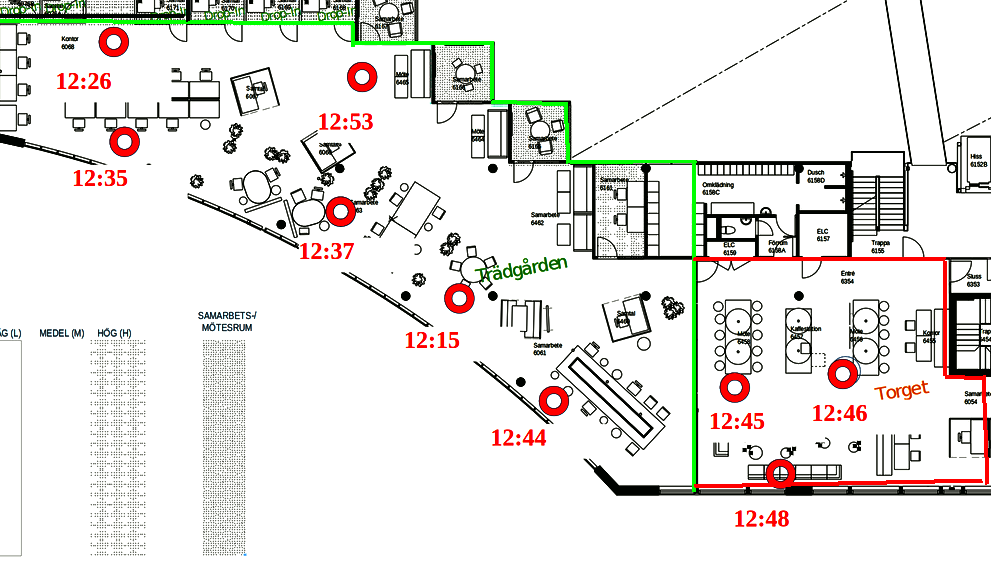
\includegraphics[width=15cm]{media/vaningstest_uppsala_kommun_2.png}}
   \caption{Våningstest på Uppsala Kommun}
   \label{fig:vanings_test}
 \end{figure}

 \begin{figure}[H]
   \centering
   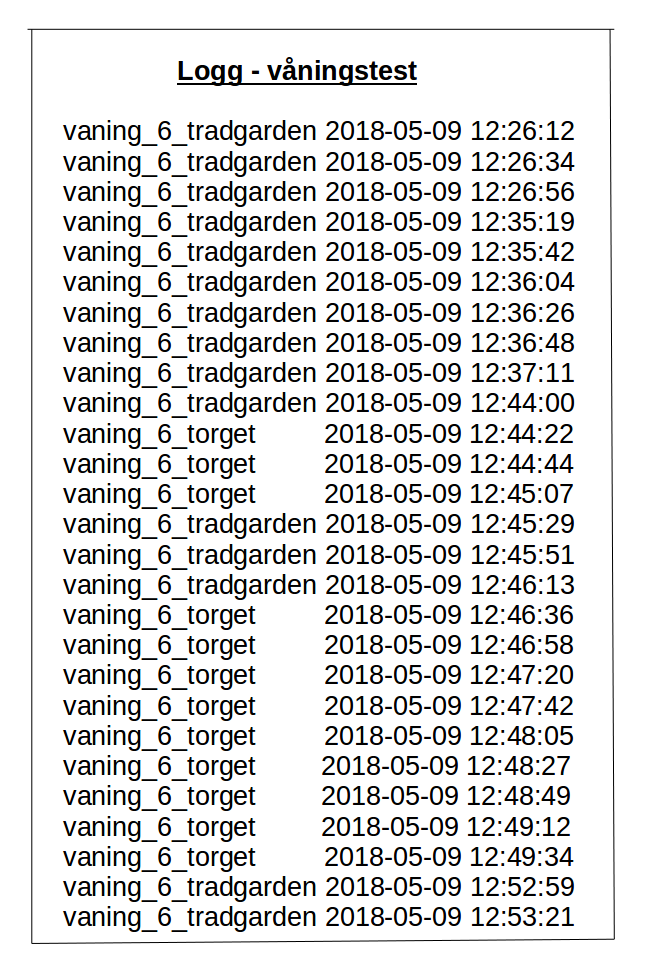
\includegraphics[width=10cm]{media/logg_vaningstest.png}
   \caption{Logg för våningstest på Uppsala Kommun}
   \label{fig:logg_vaningstest}
 \end{figure}

 Resultatet av våningstestet går att utläsa vid jämförelse av uppskattad position av systemet vid en viss tidpunkt (se loggen i figur \ref{fig:logg_vaningstest}) samt verklig position i figur \ref{fig:logg_vaningstest}. Alla positionsbestämmelser i det här testet gav en position på våning 6. Detta indikerar att systemet har förmåga att skilja på områden på olika våningsplan vilket också var vår förhoppning.

 \subsection{Områdestest hos Uppsala Kommun}
 Utöver ett våningstest utfördes även ett områdestest. Områdestestet utfördes även det på i Uppsala Kommuns lokaler på Stationsgatan 12 i Uppsala. Syftet med områdestestet var att analysera precisionen för positionsbestämningen (se sektion ~\ref{krav}). Referenspunkterna som utmättes för våningstestet (se sektion ~\ref{vaningstest}) användes även för områdestestet men utökades även med referenspunkter för fler områden på våningsplan 6. En bild på testområdet för områdestestet kan ses i figur (~\ref{fig:omrades_test}). Samma tillvägagångssätt användes vid områdestestet som vid våningstestet. De röda ringarna och tillhörande klockslag i figur ~\ref{fig:omrades_test} anger användarens position vid ett specifikt klockslag. Positionsbestämning utfördes löpande på en dator som användaren hade med sig vid varje tillfälle. Resultaten för varje positionsbestämning sparades i en logg som går att se i figur \cref{fig:logg_omradestest1,fig:logg_omradestest2}. Vid varje röd cirkel i figur ~\ref{fig:omrades_test} stannade användaren i minst en minut. Eftersom positionsbestämningen utfördes löpande på användarens medhavda dator är vissa resultat från loggningen resultat som uppkommit under användarens förflyttning mellan olika cirklar i figur ~\ref{fig:omrades_test}.

 \begin{figure}[H]
   \centering
   \fbox{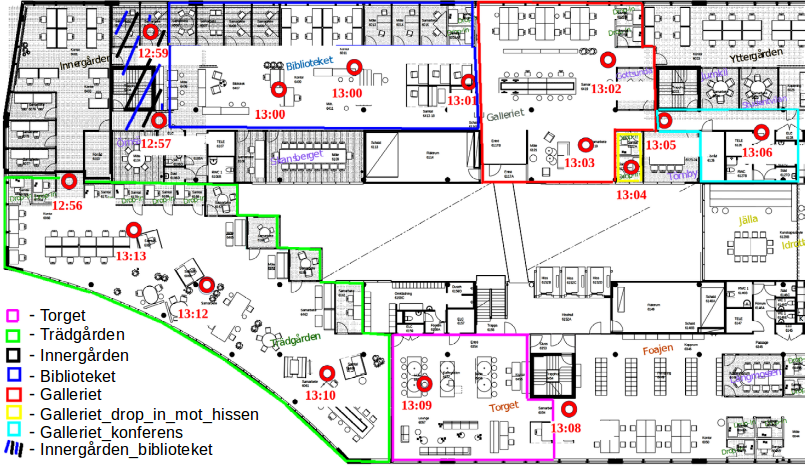
\includegraphics[width=15cm, height=13cm]{media/test_omrade_u_k.png}}
   \caption{Områdestest på Uppsala Kommun}
   \label{fig:omrades_test}
 \end{figure}

 \begin{figure}[H]
   \centering
   \fbox{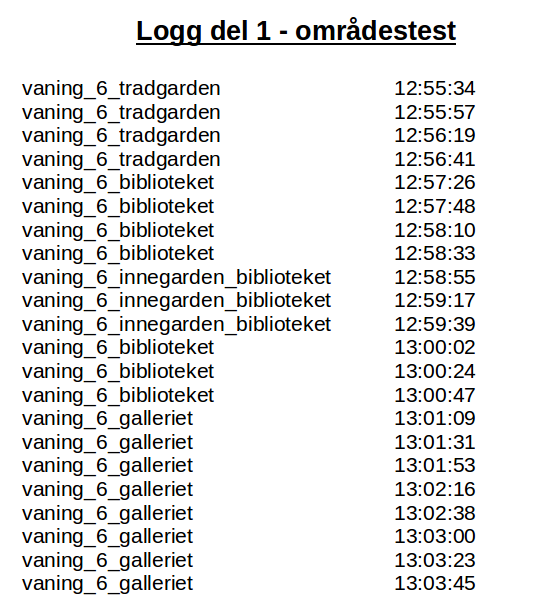
\includegraphics[width=10cm]{media/logg_omrade_del_1.png}}
   \caption{Logg del 1 efter områdestest på Uppsala Kommun}
   \label{fig:logg_omradestest1}
 \end{figure}


 \begin{figure}[H]
   \centering
   \fbox{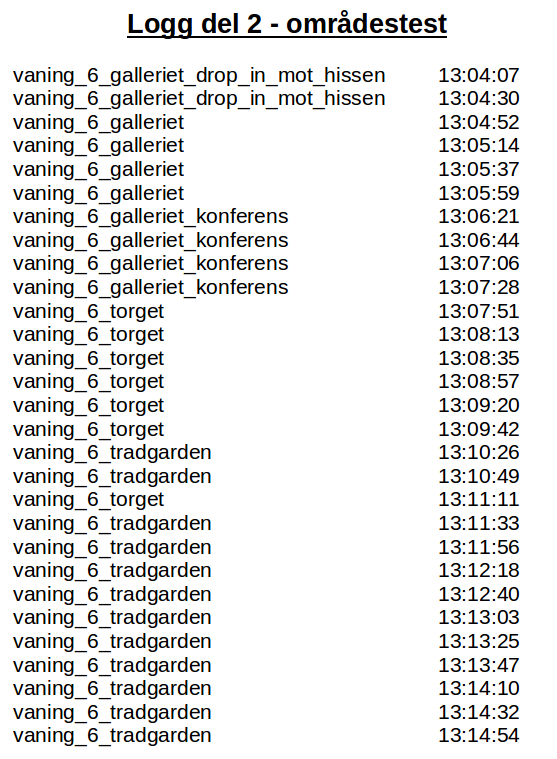
\includegraphics[width=10cm]{media/logg_omrade_del_2.png}}
   \caption{Logg del 2 efter områdestest på Uppsala Kommun}
   \label{fig:logg_omradestest2}
 \end{figure}

 Vid analys av loggarna i ~\cref{fig:logg_omradestest1,fig:logg_omradestest2} i förhållande till kartan i \cref{fig:omrades_test} uppkommer par viktiga poster i loggen som är viktiga att uppmärksamma.
 Vi kan se en tydlig felpositionering. Den uppkommer vid tidpunkt 13:11:11 i del 2 av loggen och motsvaras av cirkeln med tidpunkt 13:11 i \cref{fig:omrades_test}. Användarens position är tydligt i området Trädgården men positionsbestämningen resulterade i positionen Torget. Det är den enda uppenbara felpositioneringen som går att utläsa ur områdestestet.

 Utöver en uppenbar felpositionering går det att utläsa några felpositioneringar då användaren befinner sig precis vid en gräns mellan två områden. Några exempel på detta är:
 Positionsbestämningarna med tidpunkter mellan 13:01 och 13:02 i del 1 av loggen. Användarens position motsvaras i dessa fall av cirkeln i \cref{fig:omrades_test} med tidpunkt 13:01 angav att användaren befann sig i Galleriet. Användarens verkliga position var i dessa fall området Biblioteket men precis på gränsen till området Galleriet.
 Ett annat liknande exempel går att finna vid tidpunkterna mellan 13:05 och 13:06 i del 2 av loggen. Användarens position motsvaras i dessa fall av cirkeln i \cref{fig:omrades_test} med tidpunkt 13:05. Användarens position bestäms under detta tidsintervall till området Galleriet. Användarens verkliga position var i området \textit{Galleriet-konferens} men precis på gränsen till området Galleriet (se \cref{fig:omrades_test}).

 Utöver ett uppenbart felaktigt resultat och ett fåtal felpositioneringar som berodde på att användaren befann sig inom fem meter från gränslinje mellan två områden gav systemet för positionsbestämning enbart korrekta resultat. Totalt gjordes 51 stycken positionsbestämningar vid områdestestet. Ett fall av tydlig felpositionering innebär att vid ungefär 98\% av fallen vid områdestestet gav positionsbestämningen ett resultat med mindre felmarginal än fem meter. Tas fallen med felpositioneringar inom fem meter mot en gränslinje med i beräkningarna sjunker procentsatsen till ungefär 85\% korrekta positionsbestämmelser vid detta områdestest.

\section{Diskussion}
Eftersom detta projekt har utförts i samarbete med Uppsala Kommun har målsättningen genom hela projektet varit att utveckla ett system som de med så lite extra arbete som möjligt ska kunna integrera på deras arbetsplats. Processen för att integrera egenskriven kod, som den kod vi skrivit klassificeras som, i Uppsala Kommuns system och besår av många undersökningar och beslutsprocesser och är således en tidskrävande process. Vi har hela tiden varit medvetna om det och att det även i ett eventuellt fall med perfekta testresultat inte skulle ha varit säkert att detta system kommer att användas av Uppsala Kommun. Därav får detta projekt i vissa avseenden ses som ett ``proof of concept`` där vi visar på fördelarna som kan erhållas med ett system för inomhuspositionering på aktivitetsbaserade arbetsplatser. På grund av att angreppssättet i viss mån varit av typen ``proof of concept`` är vår förhållning till de icketekniska aspekterna vid inomhuspositionering, beskrivna i sektion \ref{icketekniska_aspekter}, som följer.

Ur ett säkerhetsmässigt perspektiv anser vi att den viktigaste funktionen vi kan bidra med är att medarbetare ska ha möjlighet att inte visa sin position. Att databasen samt systemet i övrigt är väl skyddat mot angrepp är även det viktigt men då Uppsala Kommun redan har befintliga databaser på egna servrar, vilka de även skulle använda som databas för ett positioneringssystem, anser vi att informationssäkerheten rörande databasen tillkommer Uppsala Kommun att hantera.

Ur ett etiskt perspektiv är vår ståndpunkt att syftet med det här systemet för inomhuspositionering är att det ska underlätta för medarbetarna. Alternativet är att det användas som en form av maktmedel av till exempel företagsledningen för att öka kontrollen över medarbetarna.

Utifrån den nya lagen, GDPR (se sektion \ref{GDPR}), har vi försökt utveckla systemet för att det på ett så bra sätt som möjligt ska uppfylla den nya lagen.  Den kritiska delen i systemet är att sambandet mellan en person och en plats kommer lagras i en databas och sedan presenteras för deras kollegor. Därför bör alla anställda dels kunna välja att inte finnas med i systemet över huvud taget och dels kunna välja att deras plats inte ska visas för andra. De personuppgifter som då hanteras är namn och avdelning på arbetsplatsen. Då systemet ställer dessa krav på samtycke uppfylls kraven mot GDPR i det avseendet.

Frågan om en integrering av detta system kan stöta på synpunkter från olika \\fackföreningar har vi ingen uppfattning om. Det är vår ståndpunkt att valfriheten för medarbetare och personal att använda systemet är ett val som måste erbjudas av företagsledningen eller organisationsledningen. Därmed blir också eventuella fackliga motsättningar en fråga för de personer i organisationen som beslutar om en eventuell användning av systemet.



\section{Slutsatser}
\iffalse
Här sammanfattar ni och upprepar ert bidrag (resultaten av ert projekt) och förklarar dess vikt och användning.  Vad var viktigt/nytt/intressant?  (INTE i termer av vad ni lärde er, utan för den som läser rapporten, funderar på att göra ett liknande system, vidareutveckla ert, etc.)
\fi
Vi har utvecklat ett system för inomhuspositionering med syfte att användas på aktivitetsbaserade arbetsplatser. Systemet kan positionsbestämma en användare på ett område i en lokal med en felmarginal på cirka fem meter. Enligt vår intressent, Uppsala Kommun, är detta en godtagbar precision för att systemet ska vara användbart på deras arbetsplatser. Målet med projektet har varit att underlätta för personal som arbetar på aktivitetsbaserade arbetsplatser att lokalisera varandra. Enligt de tester som vi har utfört kan det system som vi har utvecklat vara en hjälp i det avseendet.
Då detta system är är känsligt för variationer i både nätverksmiljö och fysisk struktur bör systemet testat i fler typer av både byggnader och nätverksmiljöer för att det ska vara möjligt att göra en exakt utvärdering av systemets prestanda.

Sammanfattningsvis är vi nöjda med systemets utformning och anpassning till de krav som fastställdes vid projektets början. Systemet erbjuder en möjlighet att integrera ett fungerande inomhuspositioneringssystem på en arbetsplats och som inte kräver någon extra hårdvara. För att förbättra systemet ytterligare finns många möjliga vidareutvecklingar som innefattar både presentationen av informationen i webbapplikationen samt precisionen i positionsbestämningen. Förhoppningsvis kan detta projekt ses både som ett ´´proof of concept´´ och eventuellt en grund för ett system för ska kunna fungera på en verklig arbetsplats.

\section{Framtida arbete}
\iffalse
Här beskriver ni potentiella framtida utvecklingar av systemet. Var finns förbättrings\-poten\-tial och vad kan man bygga vidare på? Vilka intressanta utvidgningar hann ni inte med?

Observera att risk\-be\-döm\-ning, tids\-planering, relation till kursmål \emph{inte} hör hemma i slutrapporten.
\fi
På grund av en begränsad tidsram för det här projektet finns många möjligheter till vidareutveckling av de olika delsystemen som ingår i detta system.

\iffalse En potentiell framtida utveckling är att i algoritmen (se sektion \ref{algoritm}) använda sig av
fler referenspunkter, dvs istället för att jämför klientenhetens närmaste \textbf{tre} referenspunkter så jämför man istället fler. Denna utveckling skulle hjälpa systemet att eventuellt klara av de gränsfall som ställs på systemet.
\fi %TODO Vi jämför med alla 10 hos klientenheten!
En möjlig vidareutveckling är att varje referenspunkt kan lagra information om fler angränsande åtkomstpunkter. Fler lagrade åtkomstpunkter för varje referenspunkt skulle leda till bättre förutsättningar för att kunna göra positionsbestämningen mer exakt. En annan möjlig vidareutveckling för att förbättra precisionen i positionsbestämningen är utföra scanningen av en och samma referenspunkt multipla gånger och med olika typer av hårdvara. För att kunna göra detta måste scanningsapplikationen utökas med stöd för fler typer av enheter. Ett annat förslag på vidareutveckling skulle kunna vara att utveckla algoritmen för positionsbestämningen så att fler metoder för positionsbestämning inkluderas. Om fler metoder inkluderas ges en större möjlighet att anpassa systemet till olika typer av byggnader där systemet kan tänkas användas.

En specifik vidareutveckling utifrån vår intressents perspektiv vore att integrera presentationen av positionsinformationen med intressentens interna medarbetarportal. Denna integrering skulle göra att medarbetarna på Uppsala Kommun inte skulle behöva använda någon annan webbtjänst än den de redan använder idag.
Ytterligare en vidareutveckling gällande presentationen av positioneringsinformationen är att föra historik över var beläggningen är som störst under vilka tidsperioder. En funktionalitet som vi ämnade utveckla var att göra det möjligt att se hur beläggningen ser ut i realtid för olika arbetsområden, därmed skulle medarbetare se var det finns gott om lediga arbetsplatser. Tyvärr hade vi på grund av tidsbrist inte möjlighet att utveckla denna ytterligare funktionalitet men vi skulle prioritera den högt i ordningen av framtida vidareutvecklingar.
\newpage
% Use one of these:
%   IEEEtranS gives numbered references like [42] sorted by author,
%   IEEEtranSA gives ``alpha''-style references like [Lam81] (also sorted by author)
\bibliographystyle{IEEEtranS}
%\bibliographystyle{IEEEtranSA}

% Here comes the bibliography/references.
% För att göra inställningar för IEEEtranS/SA kan man använda ett speciellt bibtex-entry @IEEEtranBSTCTL,
% se IEEEtran/bibtex/IEEEtran_bst_HOWTO.pdf, avsnitt VII, eller sista biten av IEEEtran/bibtex/IEEEexample.bib.
%\bibliography{bibconfig,refs} TODO: <-------Den stod från början men får det ej att funka
\bibliography{refs}

%\bibliography{refs}

\newpage
\appendix %%%% markerar att resten är appendixar
\iffalse
\section{Hur man gör appendix}
Appendixar kan vara bra för bilagor som enkätundersökningar, större kodavsnitt, etc.

Appendix läggs efter referenslistan, och ska börja på en ny sida. Använd \verb|\newpage| för att göra ett sidbrott där resten av nuvarande sida är tom. Skriv sen \verb|\appendix| för att markera att resten är appendix, och
 använd sen vanliga \verb|\section{}| för varje appendix, som kommer att ``numreras'' A, B, C osv.

\section{Några tips för La\TeX-användning}

Ett enkelt sätt att använda/\textbf{installera} LaTeX för MacOS är TexShop (\url{http://pages.uoregon.edu/koch/texshop}).

\textbf{Läs också i Wikibooks} (\url{http://en.wikibooks.org/wiki/LaTeX}), \textbf{missa inte} Appendix om ``Sample LaTeX documents'' (men använd alltid rapportmallen som bas).

\textbf{Citat-tecken} skriver man med \verb|``foo''| (dvs två bakåtfnuttar före, och två vanliga fnuttar efter). LaTeX gör så att det blir snyggt: ``foo''.

När man skriver på svenska behöver man ibland ``visa'' var ord (speciellt såna med med åäö) kan \textbf{avstavas} genom att använda \verb|\-| (liknande \textit{soft hyphen}): ämnesöversiktsintroduktion avstavas med några sådana instuckna på rätt ställen istället som ämnes\-över\-sikts\-intro\-duk\-tion

\begin{verbatim}
ämnes\-över\-sikts\-intro\-duk\-tion
\end{verbatim}

För att formattera \textbf{URLer} bättre (så att t.ex. radbrytning blir snyggare), skriv t.ex. \verb|\url{http://www.it.uu.se/research/group/concurrency}| i texten eller referensen.

För att \textbf{referera} till avsnitt, figurer, tabeller etc, använd \verb|\label{markör}| för att ``sätta ett märke'' i text eller figur, och \verb|\ref{markör}| för att referera till den, t.ex.
\begin{verbatim}
\section{Motivation}
\label{sec:motivation}
\end{verbatim}

följt av
\begin{verbatim}
Som vi nämnt i avsnitt~\ref{sec.motivation}...
\end{verbatim}

För att få referenser att inte hamna först efter ett \textbf{radbrott}, använd ``klister'' (icke-brytande space) \verb|såhär~\cite{fin-bok}|, där tilde-tecknet \verb|~| alltså gör ett obrytbart space. Detta är i princip också alltid rätt att använda före siffror, och förstås också före \verb|\ref{fig}|.

Använd \emph{aldrig} dubbel-backslash \verb|\\| för att få avbrott mellan stycken. Använd alltid dubbel ny rad för detta.

För att göra ett \textbf{sidbrott} där resten av sidan blir tom, använd \verb|\newpage|, inte \verb|\pagebreak|. Det senare är till för att finjustera var latex gör ett automatiskt sidbrott, inte för att avsluta en halvfull sida.

\subsection{Bib\TeX-tips}

För att hantera bibliografi (\textbf{referenser}) på ett smidigt sätt, använd BibTeX! (se \url{http://en.wikibooks.org/wiki/LaTeX/Bibliography_Management#BibTeX} och nedan om referenser.)

För att se till att BibTeX inte gör namn, förkortningar etc till lowercase, använd \verb|{}| och skriv typ
\begin{verbatim}
title = {The {DSP} of {N}ewton applied to {iOS}}
\end{verbatim}

Skriv alltid månader för publikation med de inbyggda förkortningarna, typ:
\begin{verbatim}
month = jun
\end{verbatim}
istället för \verb|{jun}| eller \verb|"jun"| eller \verb|"June"| eller \verb|"Juni"|. Då kan nämligen bibliographystyle styra hur det förkortas etc.

Ett verktyg för att hantera BibTeX-filer i MacOS är BibDesk (\url{http://bibdesk.sourceforge.net/}).

\section{Referenser}
\label{sec:referenser}

Se också kap 8.5 i Dawson~\cite{dawson:projects-in-computing}.

Det finns åtminstone tre syften med utformningen av referenserna och referenslistan.
\begin{enumerate}
\item Man ska hitta referensen (från texten) i referenslistan.
\item Man ska förstå vad som refereras (vilken typ av referens det är) så att man kan värdera den.
\item Man ska kunna hitta referensen i verkligheten.
\end{enumerate}

Använd numeriska referenser (IEEE-stil~[42]) eller nyckelordsbaserad~[Lam86], inte fotnotstil. Referenserna sorteras alfabetiskt efter författare/motsv i referenslistan. I LaTeX, använd \verb|\bibliographystyle{IEEEtranS}| eller \verb|{IEEEtranSA}| (eller liknande), se rapportmallen. \textbf{Börja} med att använda \verb|{IEEEtranSA}| som tydligare visar när viss info saknas i bibtex-entries (t.ex. år och författare).

För att göra inställningar för \verb|\bibliographystyle{IEEEtranS/SA}| kan man använda ett speciellt bibtex-entry \texttt{@IEEEtranBSTCTL}, se \texttt{IEEEtran\_bst\_HOWTO.pdf} i directoryt \texttt{IEEEtran/bibtex}, avsnitt VII, eller sista biten av \texttt{IEEEexample.bib} i samma directory.

Referenserna skrivs i direkt anknytning till det som föranleder referensen (t.ex. ett påstående eller resultat), före eventuellt skiljetecken, och med ett fast mellanslag till föregående ord. I La\TeX, \verb|skriv~\cite{lam86}| för att få en ``non-breaking space''. Se också rapportmallen, och sista stycket på sid 211 i Dawson~\cite{dawson:projects-in-computing}.

Det är alltså \emph{inte} en bra approach att skriva referenserna efter ett längre stycke (som vissa verkar lära sig att göra, någonstans). Det gör det oftast otydligt vad som egentligen är hämtat från, eller styrks, av referenserna. I vissa fall kan man vilka göra en kort sammanfattning av vad en författare skriver i en artikel el.dyl., men att bara lägga på en referens sist i stycket är inte tillräckligt tydligt. Det är mycket bättre och tydligare att skriva något i stil med ``Lisa Lagom beskriver\verb|~\cite{lagom-bok}| hur X beror av Y och i sin analys visar hon i detalj hur sambandet ser ut\ldots''.

När man refererar till ``tjocka'' saker som böcker är det lämpligt att ange sidnr
(som \verb|\cite[sid 211-214]{dawson}|), men för ``tunnare'' saker behöver man bara göra det för att speciellt peka ut om man t.ex. menar en viss del av referensen (kanske den tar upp tre olika sätt att göra X och man vill peka på det 3:e, inte de första två).

För mer info om vilken info som behövs för olika typer av referenser, se avsnitt 8.5.3 i Dawson~\cite{dawson:projects-in-computing,dawson:projects-in-computing-old}. (För att referera till flera saker samtidigt (som nyss) skriver man flera BibTeX-nycklar i samma \verb|\cite|.)

Använd inte direktcitat, såvida inte den exakta formuleringen är viktig.  Skriv hellre ett referat av vad någon sagt. (Se Dawson.)

Om referenslistan huvudsakligen innehåller referenser till ``mer info'' av typen
\url{www.wordpress.org}, \url{www.w3c.org}, \url{developer.android.com}\ldots men få referenser som stöder resonemang, motivation, argument etc (jfr Workshoparna), är det antagligen ett tecken på att det finns få resonemang, motiveringar och argument som behöver stödjas. Då behöver man med största sannolikhet resonera, motivera och argumentera mera!

Även om en referens har en URL till själva texten är det inte nödvändigtvis en webbreferens, utan ibland en artikel/bok el.dyl som råkar vara tllgänglig på nätet. Den ska då beskrivas som artikel/bok/el.dyl, men förstås gärna med URLen.

Försök hitta författare och publiceringsdatum (år, månad) även för webbreferenser, och ange när de lästes. Ett exempel är~\cite{berners-lee:cool-uris} (se \texttt{refs.bib}).



\section{Formler, figurer, bilder, kod}
\label{sec:forml-figur-bild}

Formler och/eller ekvationer måste beskrivas.  Det betyder t.ex. att varje symbol måste vara förklarad i texten.

I engelsk text skriver man ``Figure 3'', inte ``figure 3'', eftersom det fungerar som ett namn på figuren (och motsvarande för Table osv).

Alla figurer och bilder som inte är era egna måste ha referenser.

Figurer presenteras med en linje över, en under, och en mellan figurtexten och själva bilden. För andra presentationer, se macrot \verb|\floatstyle| (googla) -- exempelvis ger \verb|\floatstyle{boxed}| istället en ram runt figuren.

Om ni inkluderar kodsnuttar, se till att de är relevanta och kommenterade, så att man förstår.  Alternativt, för korta snuttar: ge motsvarande förklaring i texten.
Använd vettigt latex-bibliotek för kod, t.ex. \texttt{listings}.

\section{Språk och grammatik}
\label{sec:sprak-och-grammatik}

\begin{itemize}
\item    Det är OK att skriva ``Vi''!

\item    \textbf{Inte alla läsare är män}.  Skriv därför inte ``han'', ``hans'', ``denne'' etc.  Använd könsneutrala pronomen eller ord som ``vederbörande'', ``användaren'' etc.

\item    \textbf{Undvik talspråk} ``så'', ``två stycken saker'', ``ifrån'', ``utav'', ``vart'', ``kommer göra/vara'' (istället för ``kommer att göra/vara'', \ldots \textbf{Kolla på Wikipedia-sidan} ``Vanliga språkfel'' (länk i vänsterkanten i SP).

\item    Undvik värderande uttryck som enkelt, uppenbart.

\item    Semikolon är \textbf{inte} en variant av kolon eller komma; semikolon kan endast användas där ni normalt sett skulle använt punkt, men vill fortsätta på samma mening. För att undvika problem, undvik semikolon helt.

\item    Skriv inte meningar som börjar med ``Detta på grund av'' eller ``Detta eftersom\ldots' -- det blir ofta inte fullständiga meningar och det är ofta inte klart vad ``detta'' syftar på.

\item    Använd inte framtid; skriv rapporten i nu- eller dåtid och var konsekventa (Vi gör\ldots eller Vi har gjort\ldots, inte Vi kommer att göra\ldots)

\item    \textbf{Förklara begrepp innan ni använder dem}, hänvisa inte \emph{bara} läsaren till ett senare avsnitt (men ni kan naturligtvis också hänvisa till mer detaljerade förklaringar som kommer senare i texten).  Första gången ett begrepp nämns måste alltså åtminstone en kort förklaring finnas.

\item    När ni introducerar nya koncept (sådant ni inte har diskuterat tidigare), gör inte det ``i förbifarten'', utan se till att ni \textbf{förklarar ordentligt}.  Alltså: ``Vi använder X (ett häftigt nytt programmeringsspråk) för att göra Y'' fungerar inte.  Beskriv först konceptet ni använder, och använd det sedan.  Typ ``X är ett viktigt nytt programmeringsspråk.  Vi använder X för att göra Y.''

\item    \textbf{Var konsekventa} med hur ni skriver förkortningar och begrepp (c++ eller C++, android och Android t.ex.) Tumregel: namn skrivs med inledande stor bokstav (Android, inte android), förkortningar med stora bokstäver (XML, inte Xml).
\item    Använd inte olika synonymer för det ni har utvecklat (tjänsten/projektet/systemet), utan bestäm er för vad det är ni har gjort.

\item    Det kan vara bra att kursivera nya begrepp första gången de används, men normalt bör man inte kursivera \emph{alla} förekomster.

\item    Efter uttryck som ``för det första\ldots'', ``one alternative is\ldots'' måste följa ``för det andra\ldots'' ``another alternative'' (inte ``slutligen'', ``dels'', ``another \underline{option}'' eller något annat).  Tänk också på ``firstly \ldots secondly'' resp. ``first \ldots second'', inte ``first \ldots secondly'' eller något annat.

\item    Var försiktig med uttryck som ``this approach'', ``detta system'', etc. och kontrollera att det är uppenbart vad detta/this refererar till. Be någon icke-gruppmedlem läsa och kolla!

\item    De av er som skriver på engelska: ni MÅSTE använda korrekta verbformer beroende på om subjektet är en eller flera saker (``it has'' men ``they have'').
\end{itemize}
\fi

\end{document}
